\chapter{Background Estimations and Uncertainties}
\label{ch:bg_estim}
A discussion of the dominant backgrounds, their uncertainties and their estimations are inseparably linked to the complicated statistical calculations performed to estimate a limit on the cross-section of a possible \WR. This chapter serves as the first of two discussing the approaches of this analysis therein. Here, dominant backgrounds and their dominant uncertainties are discussed in detail and the remaining uncertainties briefly explained. Section~\ref{ch:limit_setting} delves into statistical techniques and calculations used in this chapter and presents the resulting limit 

\section{Primary Background Estimations}
Both \ttbar and \Zg can have the same final state as the signal and they are the main sources of background in both the resolved and boosted regions of this analysis. There are several other backgrounds also accounted for in this analysis, however, they occur at a low enough rate to both have a much smaller overall contribution and prove to difficult to directly study. These backgrounds are estimated directly from Monte-Carlo simulations. In order to better-estimate the two dominant backgrounds, \ttbar and \Z+Jets, two control regions defined in Chapter~\ref{ch:strategy} are used. As each year's Monte-Carlo has its own corrections and is partially correlated with the other years, each year's distribution for each background is handled separately for the purposes of limit-setting. However, where possible each year is shown stacked with the others for simplicity.

\subsection{Drell-Yan}
To estimate the background from high-mass or high-\pt Drell-Yan lepton pairs produced in association with additional jets, a leading order (LO) MC simulation is used. While this simulation produced ample events to make a statistically precise estimate of the Drell-Yan background in our signal region, there are a few ways in which the simulation has been observed to be inconsistent with data (and in the control region of this analysis simulation additionally deviates after initial correction). The spectrum of all Monte-Carlo events in the Drell-Yan control region (described in Section~\ref{sec:DYSB}) is shown in Fig.~\ref{fig:DYCR_preAll}.
In the Drell-Yan control region, the simulated \pt of the \Z boson deviates from data. To correct this issue, a \pt correction was derived by reweighting Drell-Yan simulation based on next-to-leading-order (NLO) Drell-Yan simulation. While it is certain that the NLO simulation better agrees with measurements in the Drell-Yan control region, it is assumed that this relationship holds true in the signal region as well. These corrections are shown in Fig.~\ref{fig:BkgdZptReweight}.
\begin{figure}[htbp]
  \centering

  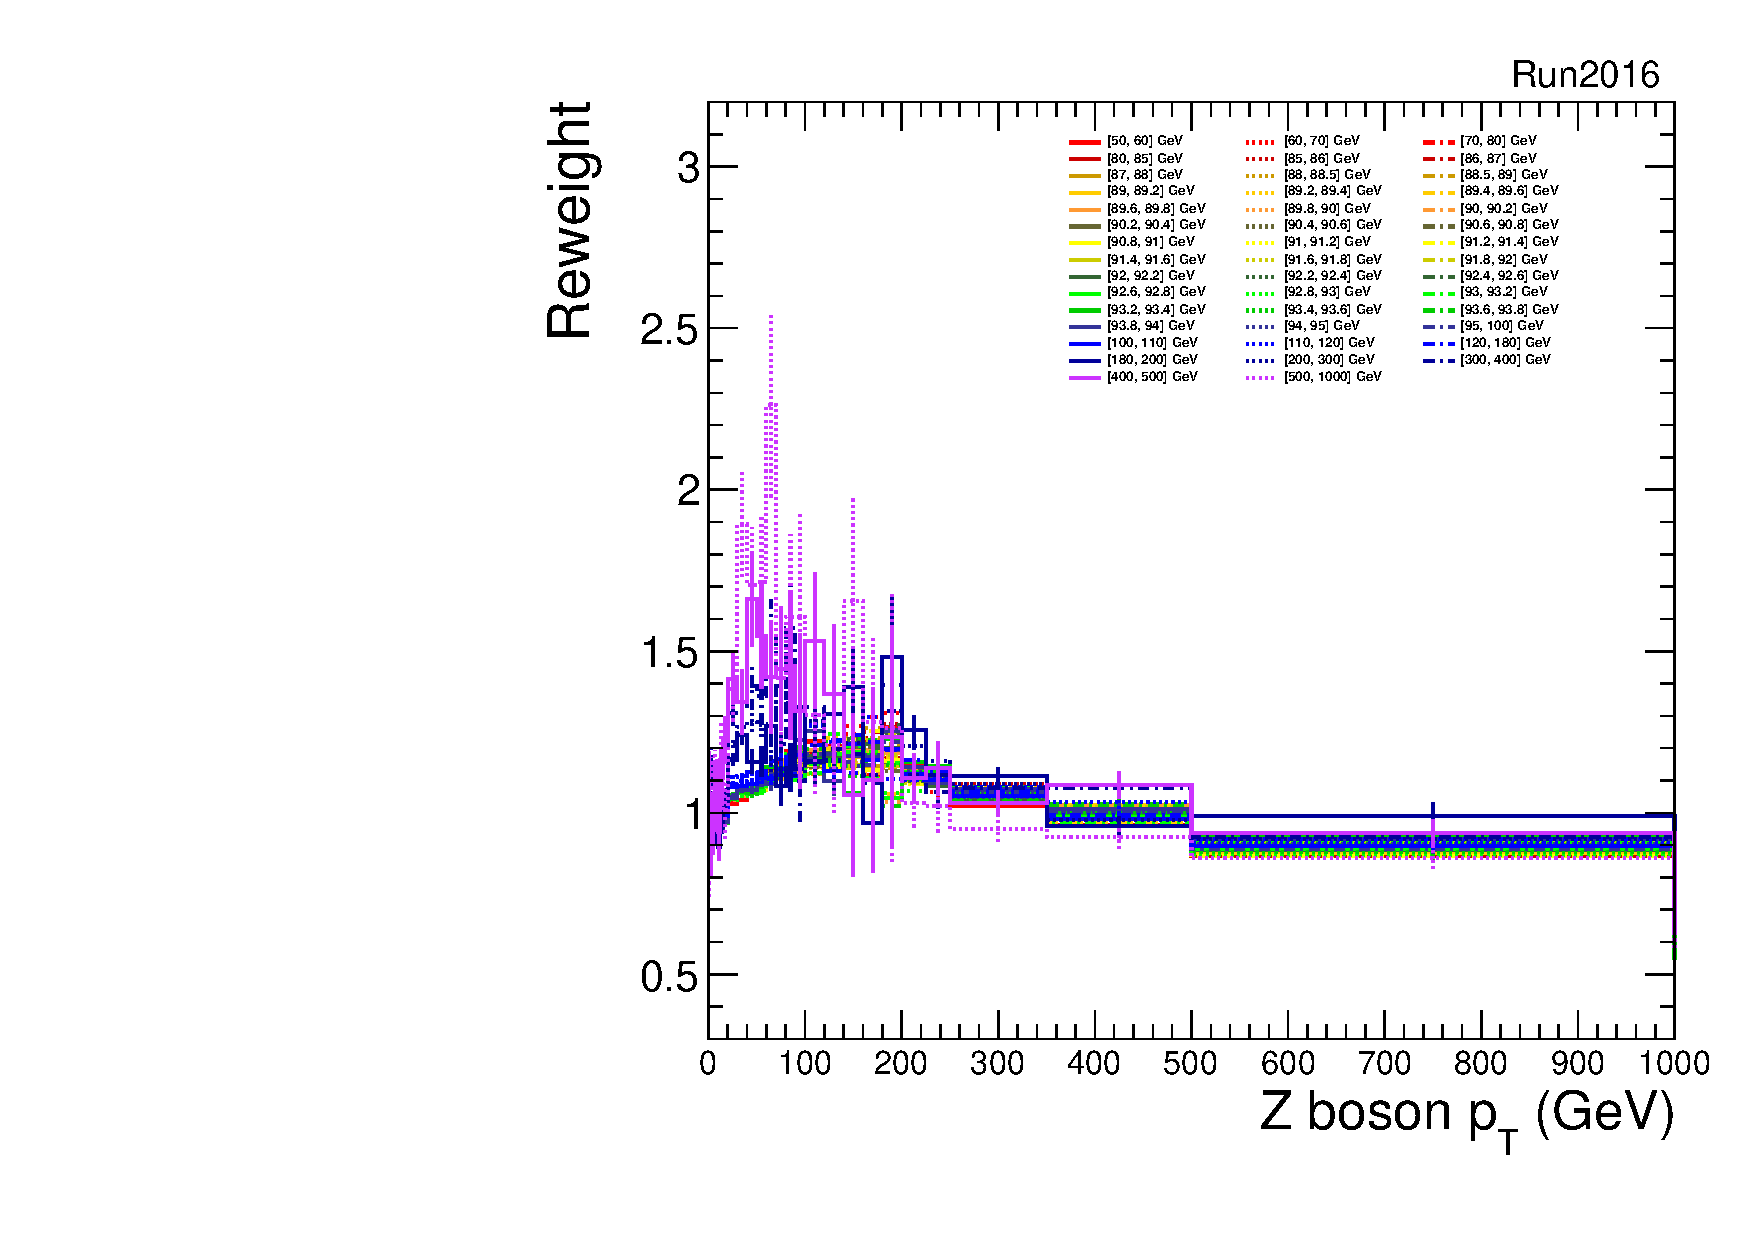
\includegraphics[width=0.45\textwidth]{figures/2016/Reweights_2016.pdf}
  \hspace{0.01\textwidth}

  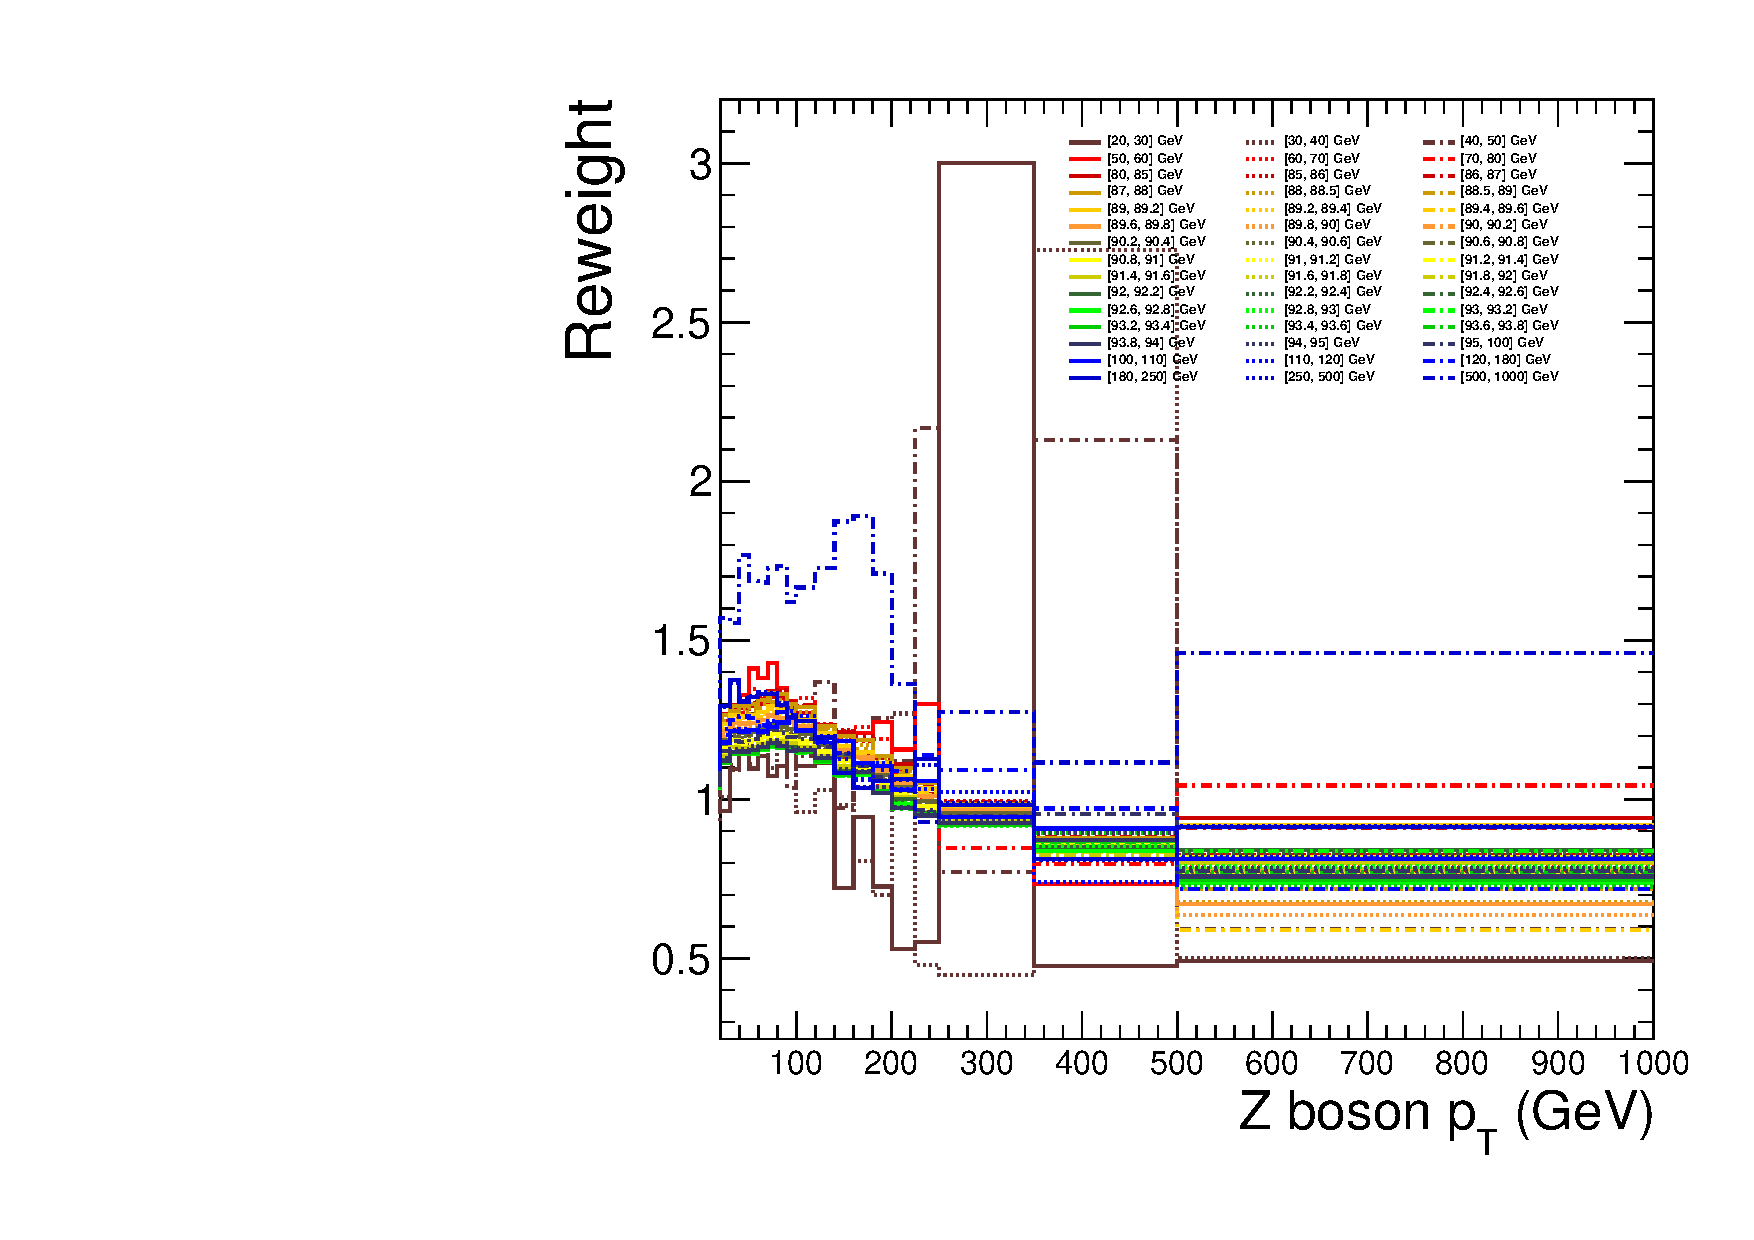
\includegraphics[width=0.45\textwidth]{figures/2017/Reweights_2017.pdf}
  \hspace{0.01\textwidth}

  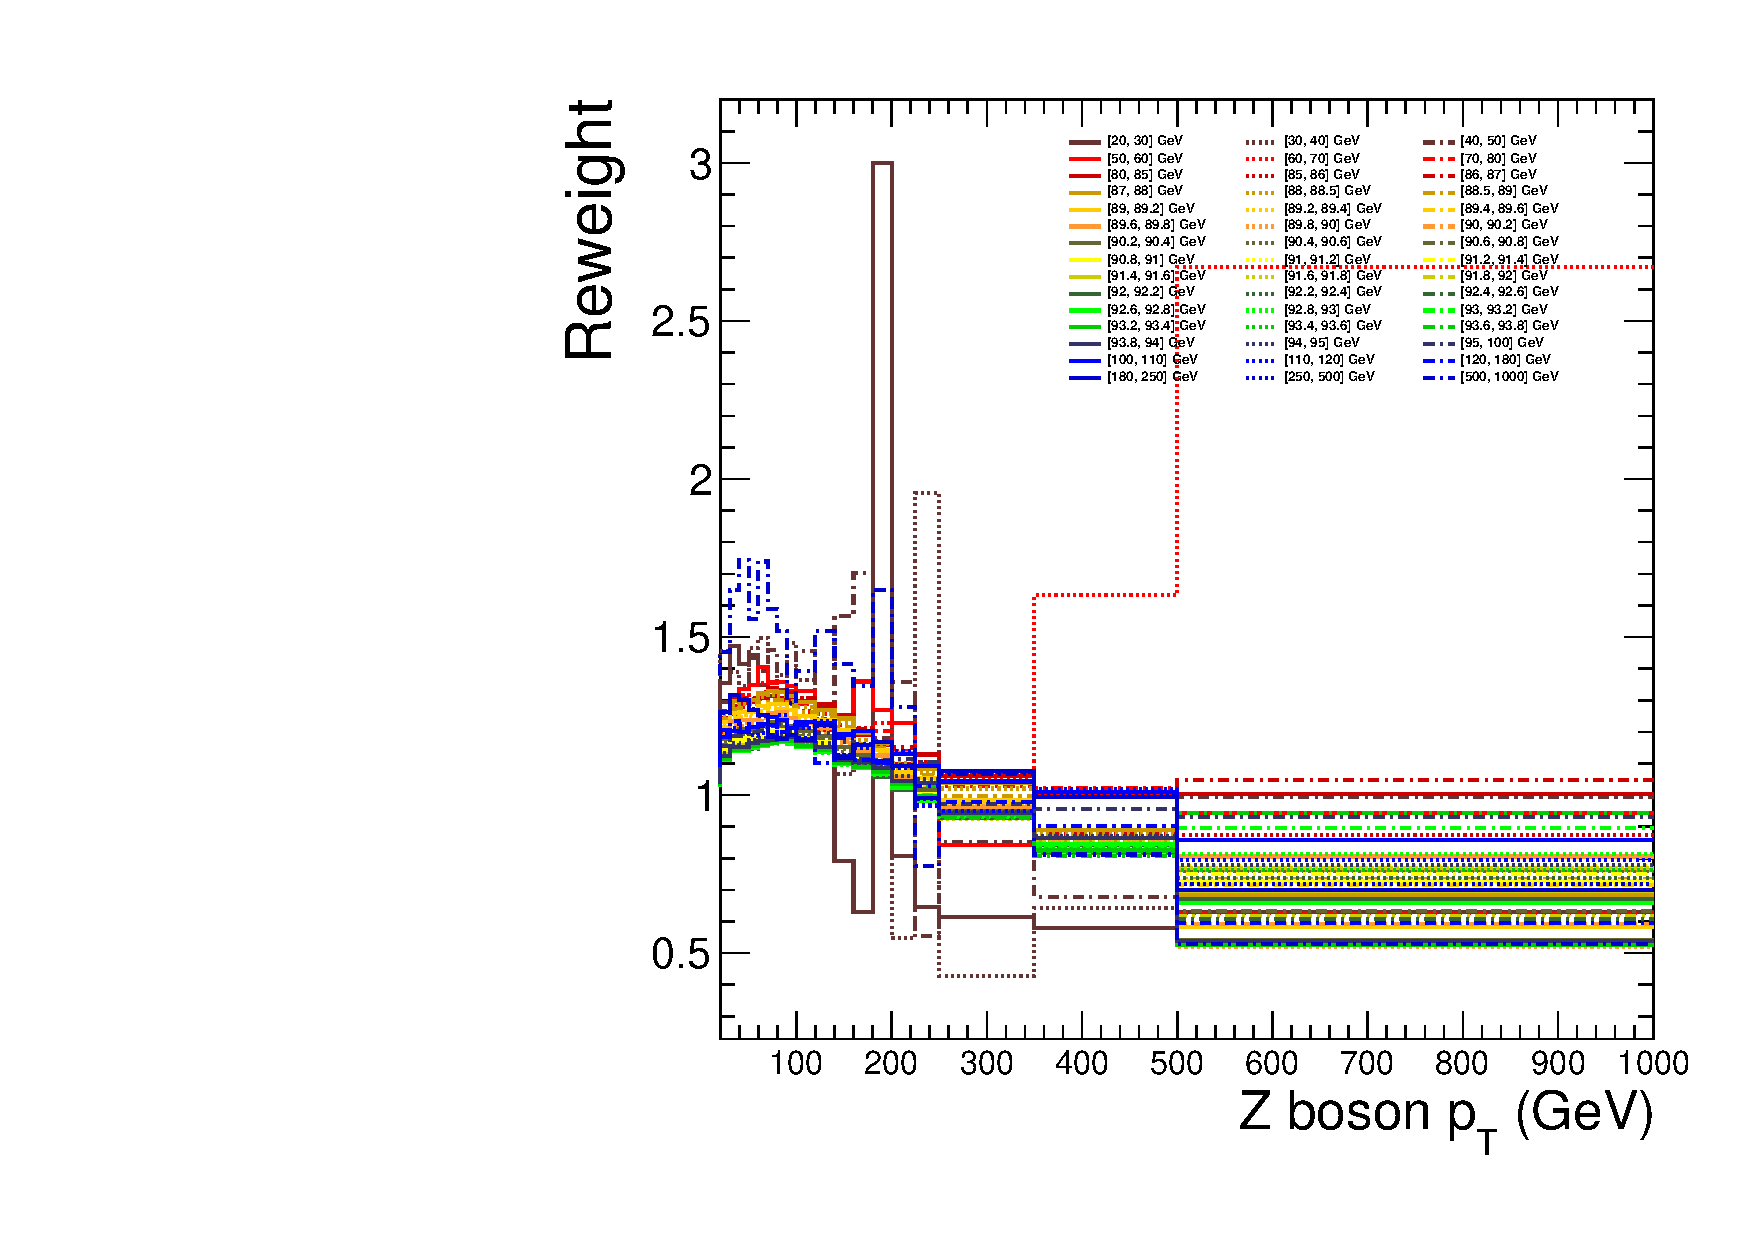
\includegraphics[width=0.45\textwidth]{figures/2018/Reweights_2018.pdf}

  \topcaption{
    The \Z-\pt-mass correction functions, for 2016 (upper), 2017 (middle) and 2018 (lower)~\cite{CMS-PAS-SMP-15-011}.
  }
  \label{fig:BkgdZptReweight}
\end{figure}

After these corrections an observed difference remains between the Drell-Yan and data in the Z-mass sideband in the resolved signal mass spectrum. The LO samples used in this analysis over-predict the data distribution noticeably. The difference between data and Monte-Carlo for both lepton flavors is shown in Fig.~\ref{fig:LO_Z_vs_data}. As LO and next-to-leading order (NLO) Monte-Carlo simulate a different number of partons, it is important to consider the NLO spectrum as well. The NLO and LO spectra (with and without Z-\pt reweighting) are shown in Fig.~\ref{fig:DYCR_NLOvLO}. The spectrum of the highest \pt jet in the selection region is shown alongside the signal mass spectrum. From the jet \pt distribution its clear that the LO jet distribution is consistently harder in the high \pt tail as might be expected. While there are differences between the shape of this difference between the two lepton flavor selections, these are assumed to be fluctuations. The correction is calculated combining the two flavors.


\begin{figure}[!tp]

  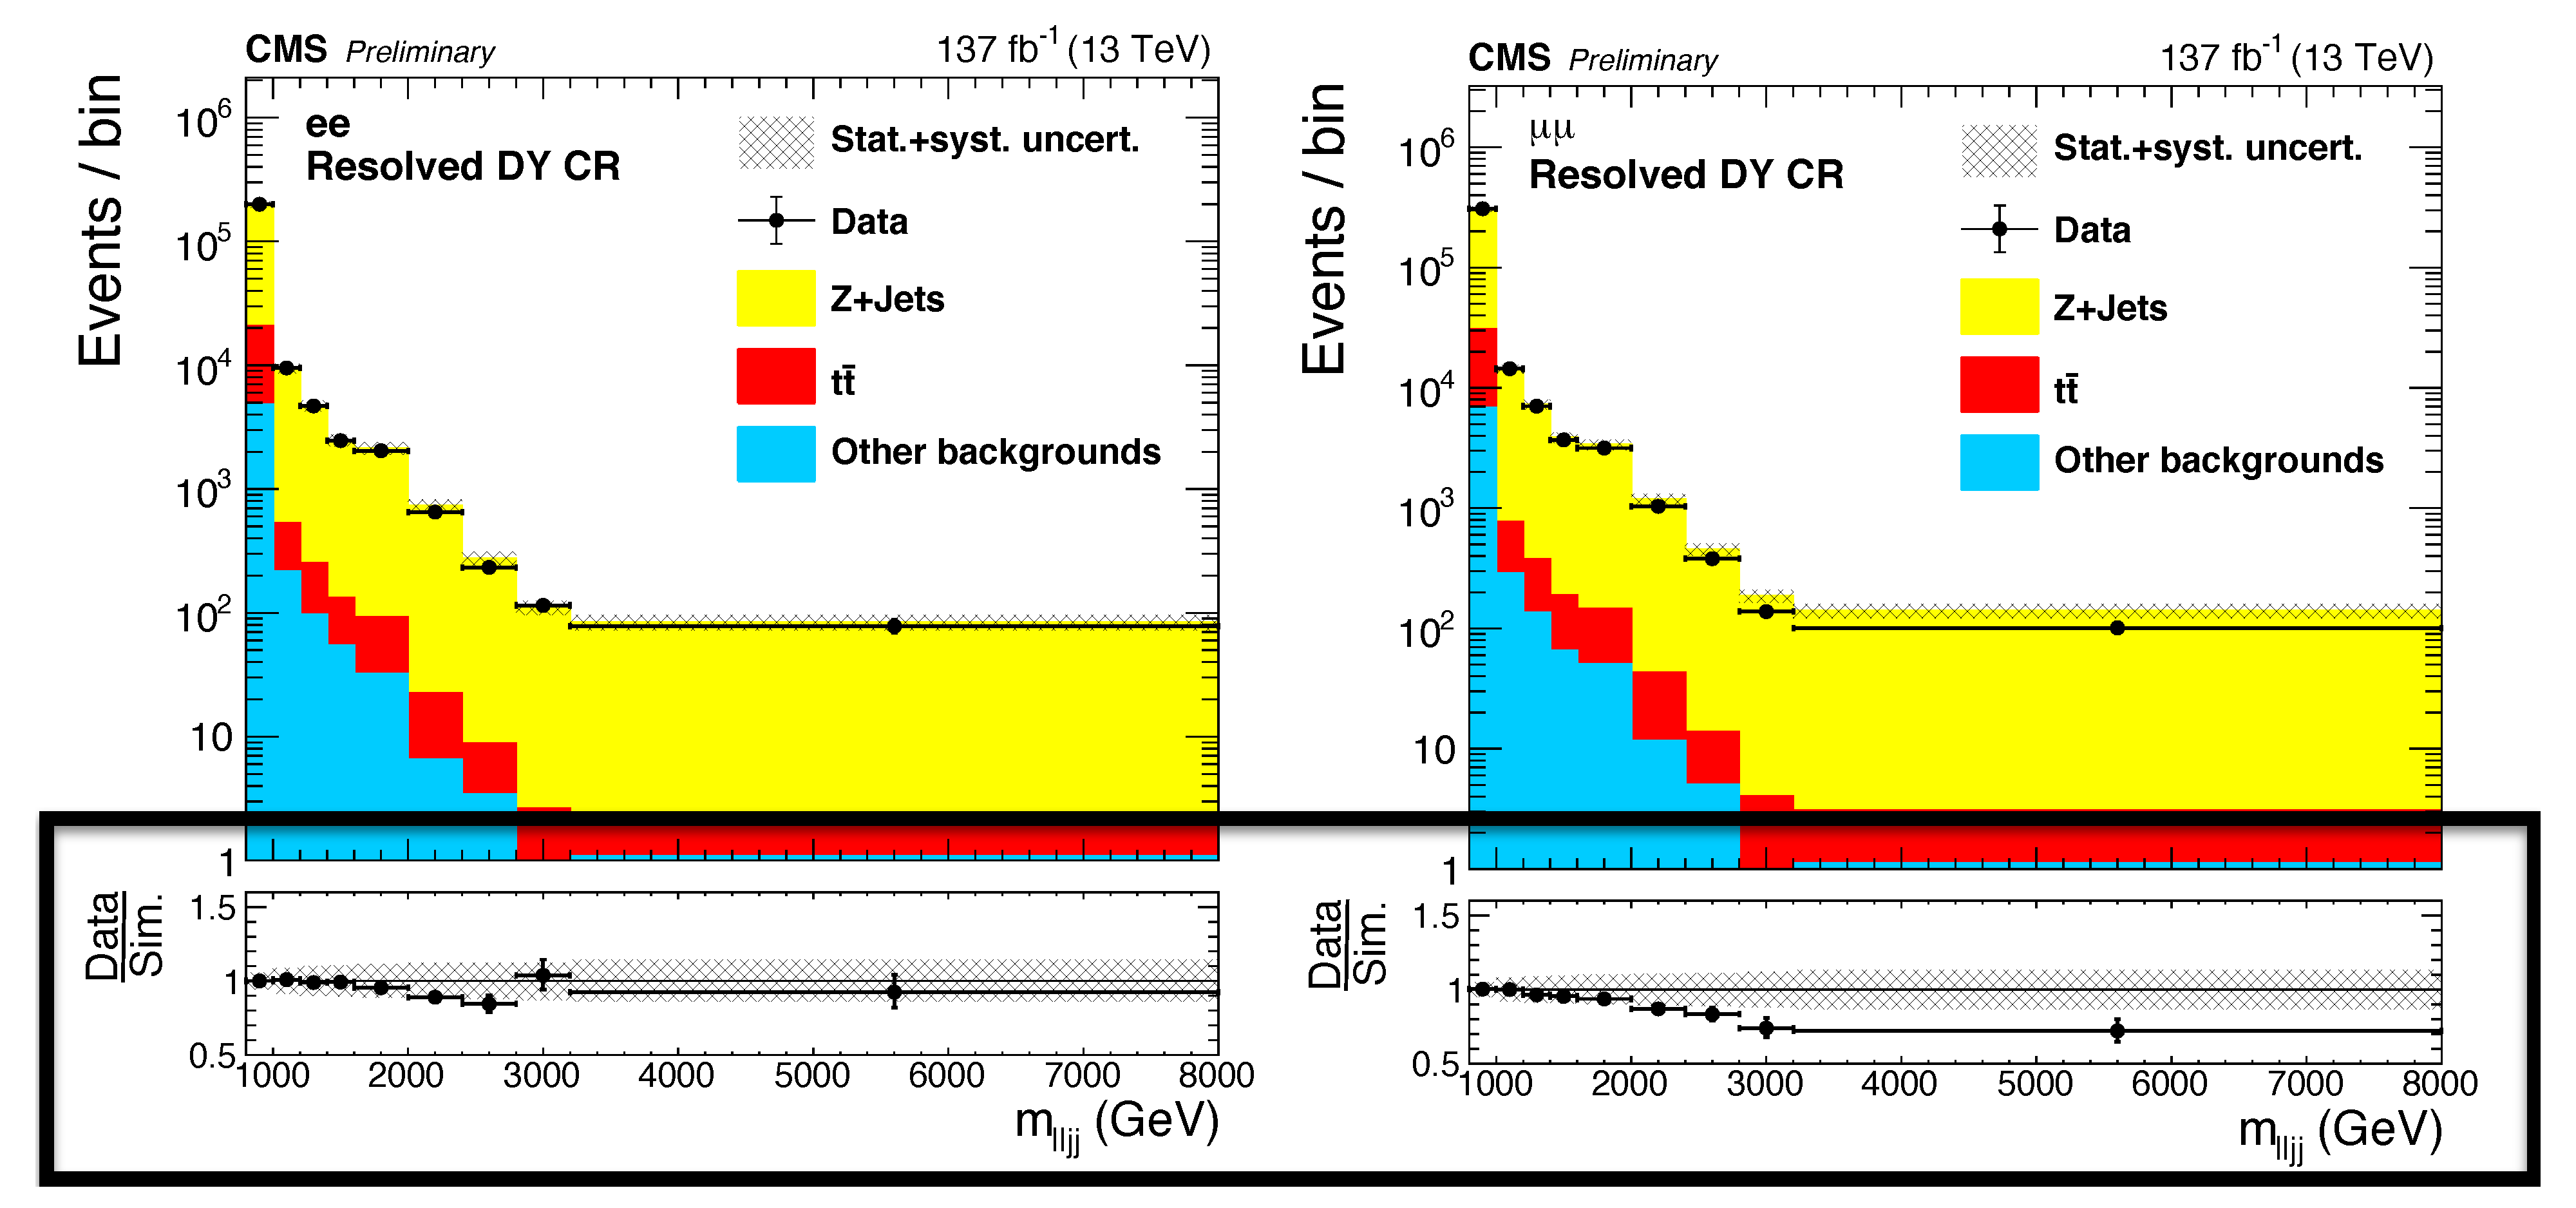
\includegraphics[width=\textwidth]{figures/DYCR_wrmass.pdf}

  \caption[Drell-Yan Data vs Monte-Carlo]{
    Data and Monte-Carlo in the Z-mass sideband are compared in the electron and muon flavors shown on the left and right, respectively. Data over Monte-Carlo is highlighted and shown in the bottom two plots.
  }
  \label{fig:LO_Z_vs_data}
\end{figure}

\begin{figure}[!tp]

  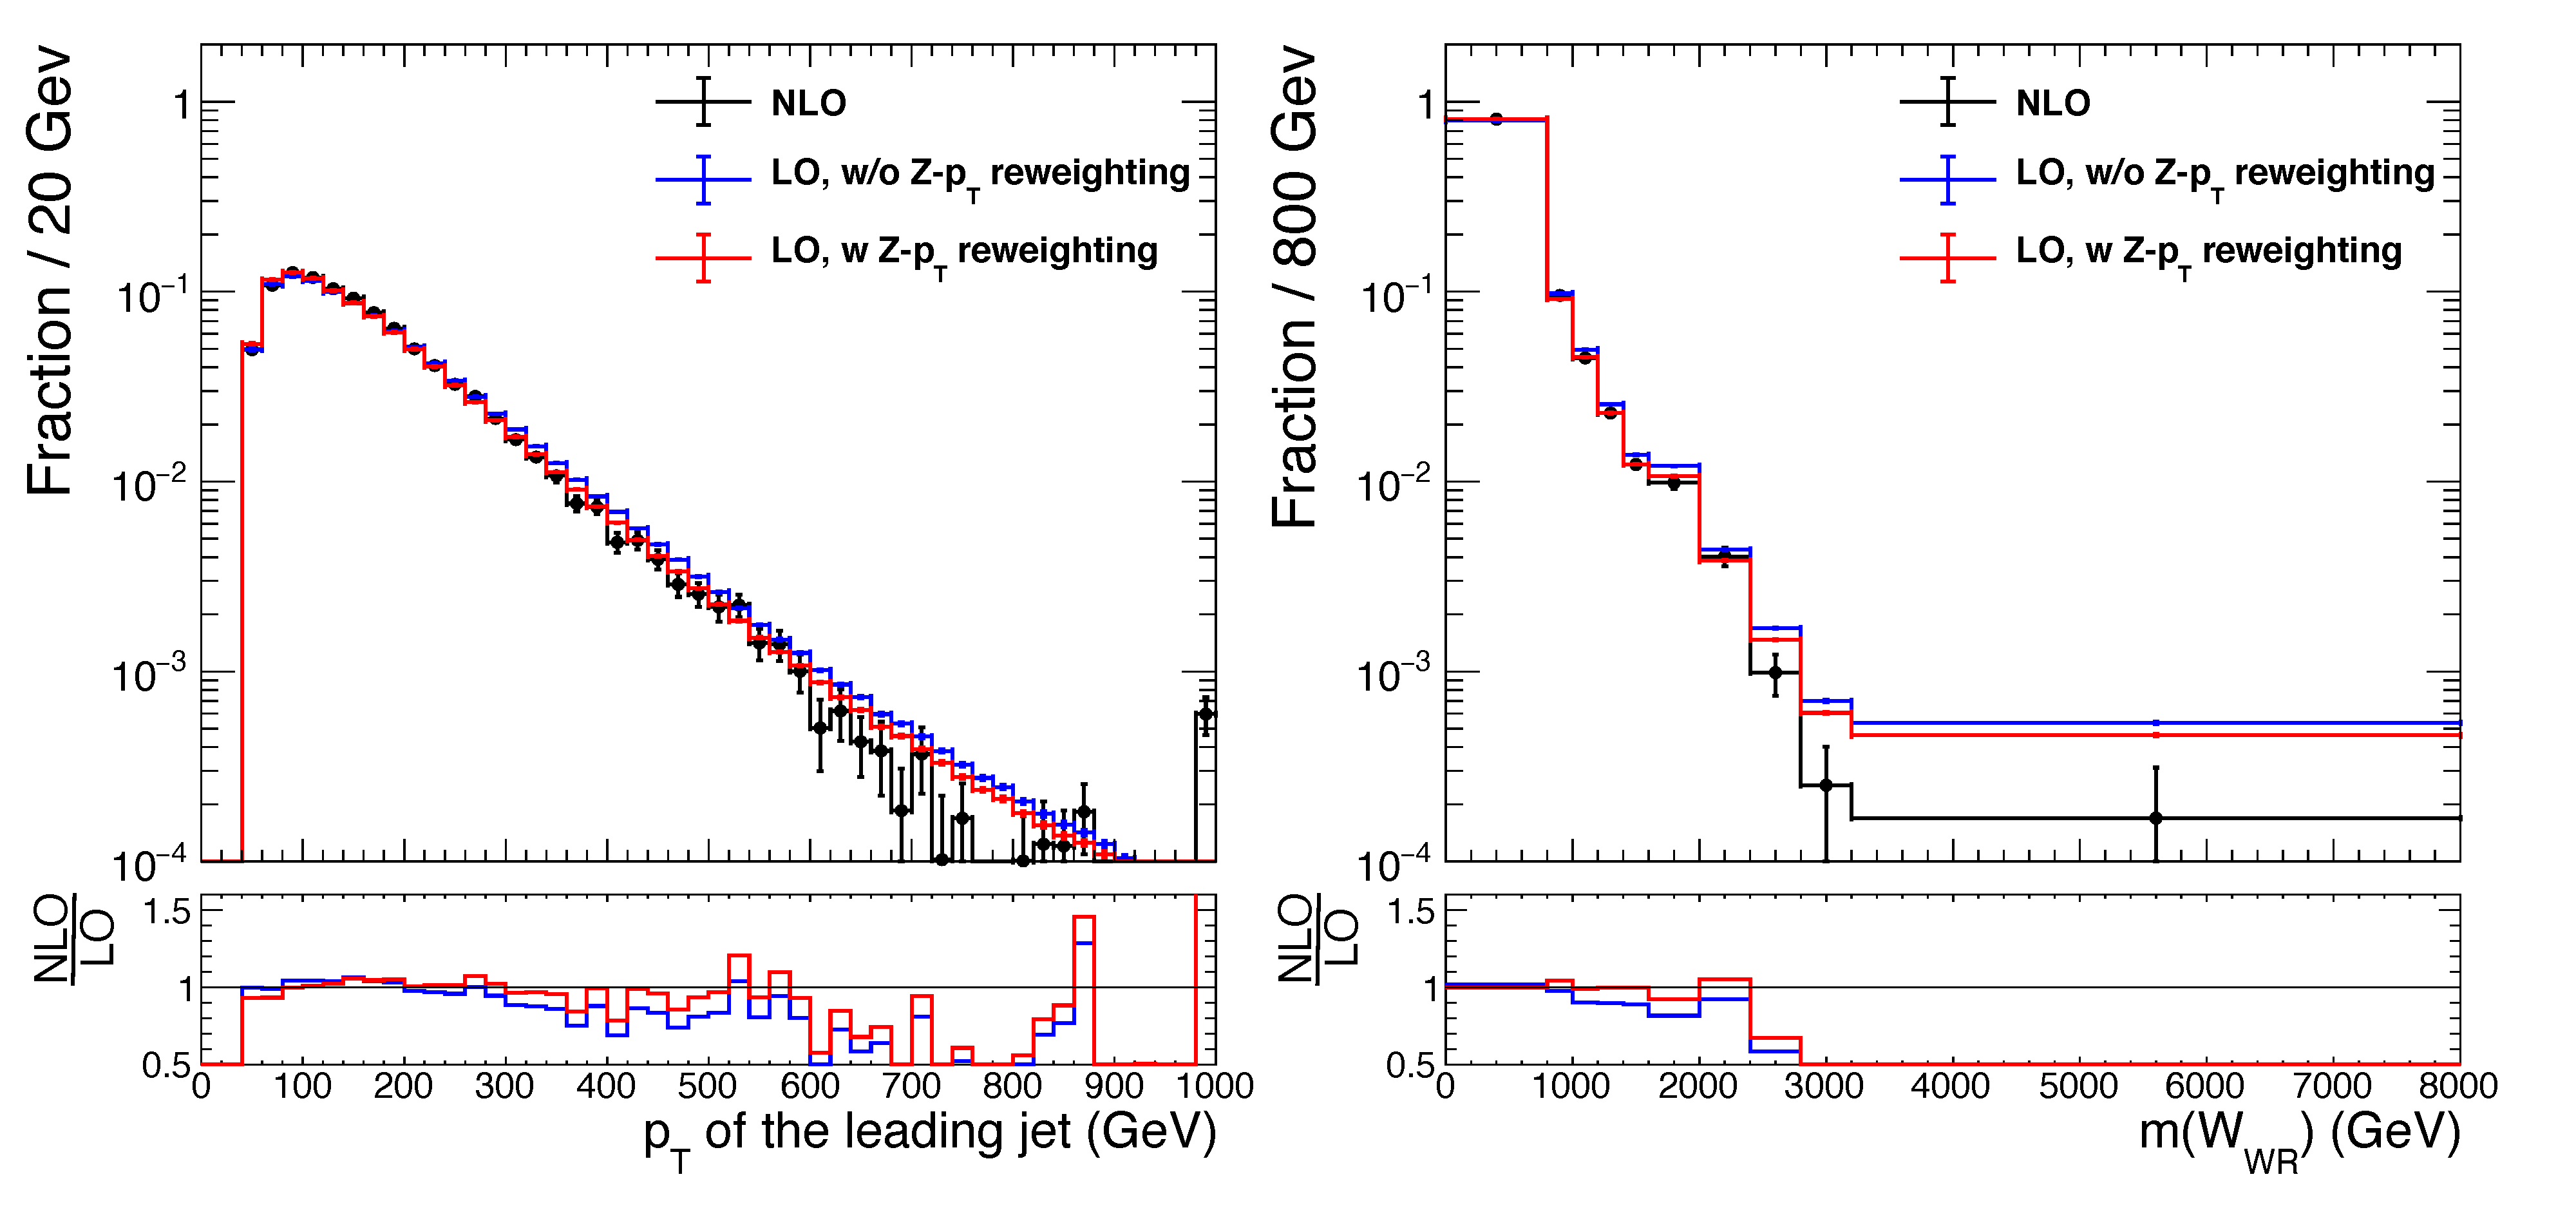
\includegraphics[width=\textwidth]{figures/DYCR_NLOvLO.pdf}

  \caption[Drell-Yan LO versus NLO spectra]{
    The spectra of simulated Drell-Yan are compared at LO with and without reweighting and NLO. The highest-\pt jet spectrum is shown on the left, and the signal mass is shown on the right.
  }
  \label{fig:DYCR_NLOvLO}
\end{figure}

We hypothesize that the discrepancy in \WR mass observed is due to QCD effects which are independent of the Drell-Yan invariant mass.
A bin-by-bin correction factor ($\xi_{i}$) is calculated in this control region and applied to the LO Drell-Yan simulation in all regions. The correction factor is calculated in two steps, first the ratio of Drell-Yan in data and Monte-Carlo is calculated:
\begin{equation}
    \xi_{i}
    =
    \frac{\mathrm{DY_{NLO}}}{\mathrm{DY_{LO}}}.
\end{equation}
This ratio is calculated fore each reconstructed \WR candidate mass bin, in each year, for the boosted and resolved Drell-Yan control regions. The muon and electron flavors, however, are combined, as the jet hardness simulated will be independent of lepton flavor. As other simulation, reconstruction and selection differences between the two lepton flavors may also occur, an additional uncertainty is added which is formed with the difference between the ratio if calculated with electron or muon events separately. These two corrections are then applied to the Drell-Yan in the signal region.

\todo{plot of the DY signal region}

\subsection{ttbar+jets background estimation}
\label{sec:ttbarBkgd}

The \ttbar background contribution is estimated with Monte-Carlo with an additional normalization factor that is calculated by performing a simultaneous fit of constant scale applied on every bin, in all regions.

%The \ttbar background contribution is estimated directly from data in the flavor sideband CR, which has the same kinematics as the \ttbar in the signal region.
%The contribution from other backgrounds in this CR are taken from simulation and subtracted from the data to produce a pure \ttbar sample.
%For this estimate, the assumption made on the conservation of the flavor in the decay is needed to ensure that there is no contamination from signal events.
%Thus, the decay of a real $\PWR$ boson at leading order cannot yield an $\Pe\mu$ final state and the flavor sideband is dominated by $\ttbar$ events.
%To calculate the number of events from \ttbar in the muon signal region, for both the boosted and resolved analyses, we used the \ttbar Monte-Carlo to find the SFs $R_{\Pe\mu/\mu\mu}$ between the flavor sideband and the signal regions.
In each region, the normalization ($\Xi_{r}$) is calculated by subtracting the simulated \ttbar distribution from the data and compared with the \ttbar simulation alone. The simultaneous fit attempts to find the normalization $\Xi$ which best agrees with the measured ratios in each region. This is used to scale the \ttbar in all regions.
\begin{equation}
    \Xi_{r}
    =
    \frac{\mathrm{Data_{r}}-\mathrm{MC_{other,r}}}{\mathrm{MC_{\ttbar,r}}}.
\end{equation}
The normalization factors for \ttbar are shown in Table~\ref{tab:EMuRatioFit}.
\begin{table}[htbp]
  \caption{
    The fitted rate parameter of \ttbar background.
  }
  \centering


  \begin{tabular}{cccc}

\hline
Year & Event type & Fitted with $ee$ SRs & Fitted with $\mu\mu$ SRs \\
\hline

\multirow{3}{*}{2016} & Resolved & $0.98 \pm 0.05$ & $0.95 \pm 0.05$ \\
                      & Boosted with $e$-Jet & $0.86 \pm 0.12$ & $0.85 \pm 0.12$ \\
                      & Boosted with $\mu$-Jet & $0.77 \pm 0.10$ & $0.76 \pm 0.09$ \\
\multirow{3}{*}{2017} & Resolved & $1.05 \pm 0.05$ & $1.04 \pm 0.05$ \\
                      & Boosted with $e$-Jet & $0.99 \pm 0.13$ & $0.94 \pm 0.13$ \\
                      & Boosted with $\mu$-Jet & $0.92 \pm 0.11$ & $0.91 \pm 0.11$ \\
\multirow{3}{*}{2018} & Resolved & $1.00 \pm 0.04$ & $1.00 \pm 0.04$ \\
                      & Boosted with $e$-Jet & $0.89 \pm 0.10$ & $0.86 \pm 0.10$ \\
                      & Boosted with $\mu$-Jet & $0.68 \pm 0.08$ & $0.78 \pm 0.08$ \\

\hline
  \end{tabular}
\label{tab:EMuRatioFit}
\end{table}




\section{Systematic Uncertainties}

The systematic uncertainties in this analysis are meant to cover a wide range of discrepancies between data and simulation. This section divides the systematic uncertainties into categories. Each systematic uncertainty is ultimately propagated through to the final \WR mass distribution in various ways. As is discussed in Chapter~\ref{ch:limit_setting}, every systematic uncertainty is calculated in every signal region and sideband.

\subsection{Background Driven Uncertainties}
\subsubsection{\ttbar}
The dominant uncertainty for the \ttbar background is on the normalization of \ttbar simulation. This normalization is calculated simultaneously in each region, with the flavor sideband having the strongest influence.

\subsubsection{Drell-Yan}
There are three dominant systematic uncertainties affecting the Drell-Yan simulations. The first is the uncertainty in the Z \pt-mass reweighting. This uncertainty varies, but is largest in the highest \pt and mass region at $30\%$. The second and third dominant uncertainties come from the residual data and simulation discrepancy noticed in the control region. As mentioned earlier, the uncertainty on the nominal value of the ratio is calculated per bin and includes all of the statistical and other systematic uncertainties. As there is some difference between the nominal value when calculated with the two lepton flavors separately, their difference is included as a systematic uncertainty. A diagram of these two uncertainties is shown in Fig.~\ref{fig:DYCR_ratio}

\begin{figure}[!tp]

  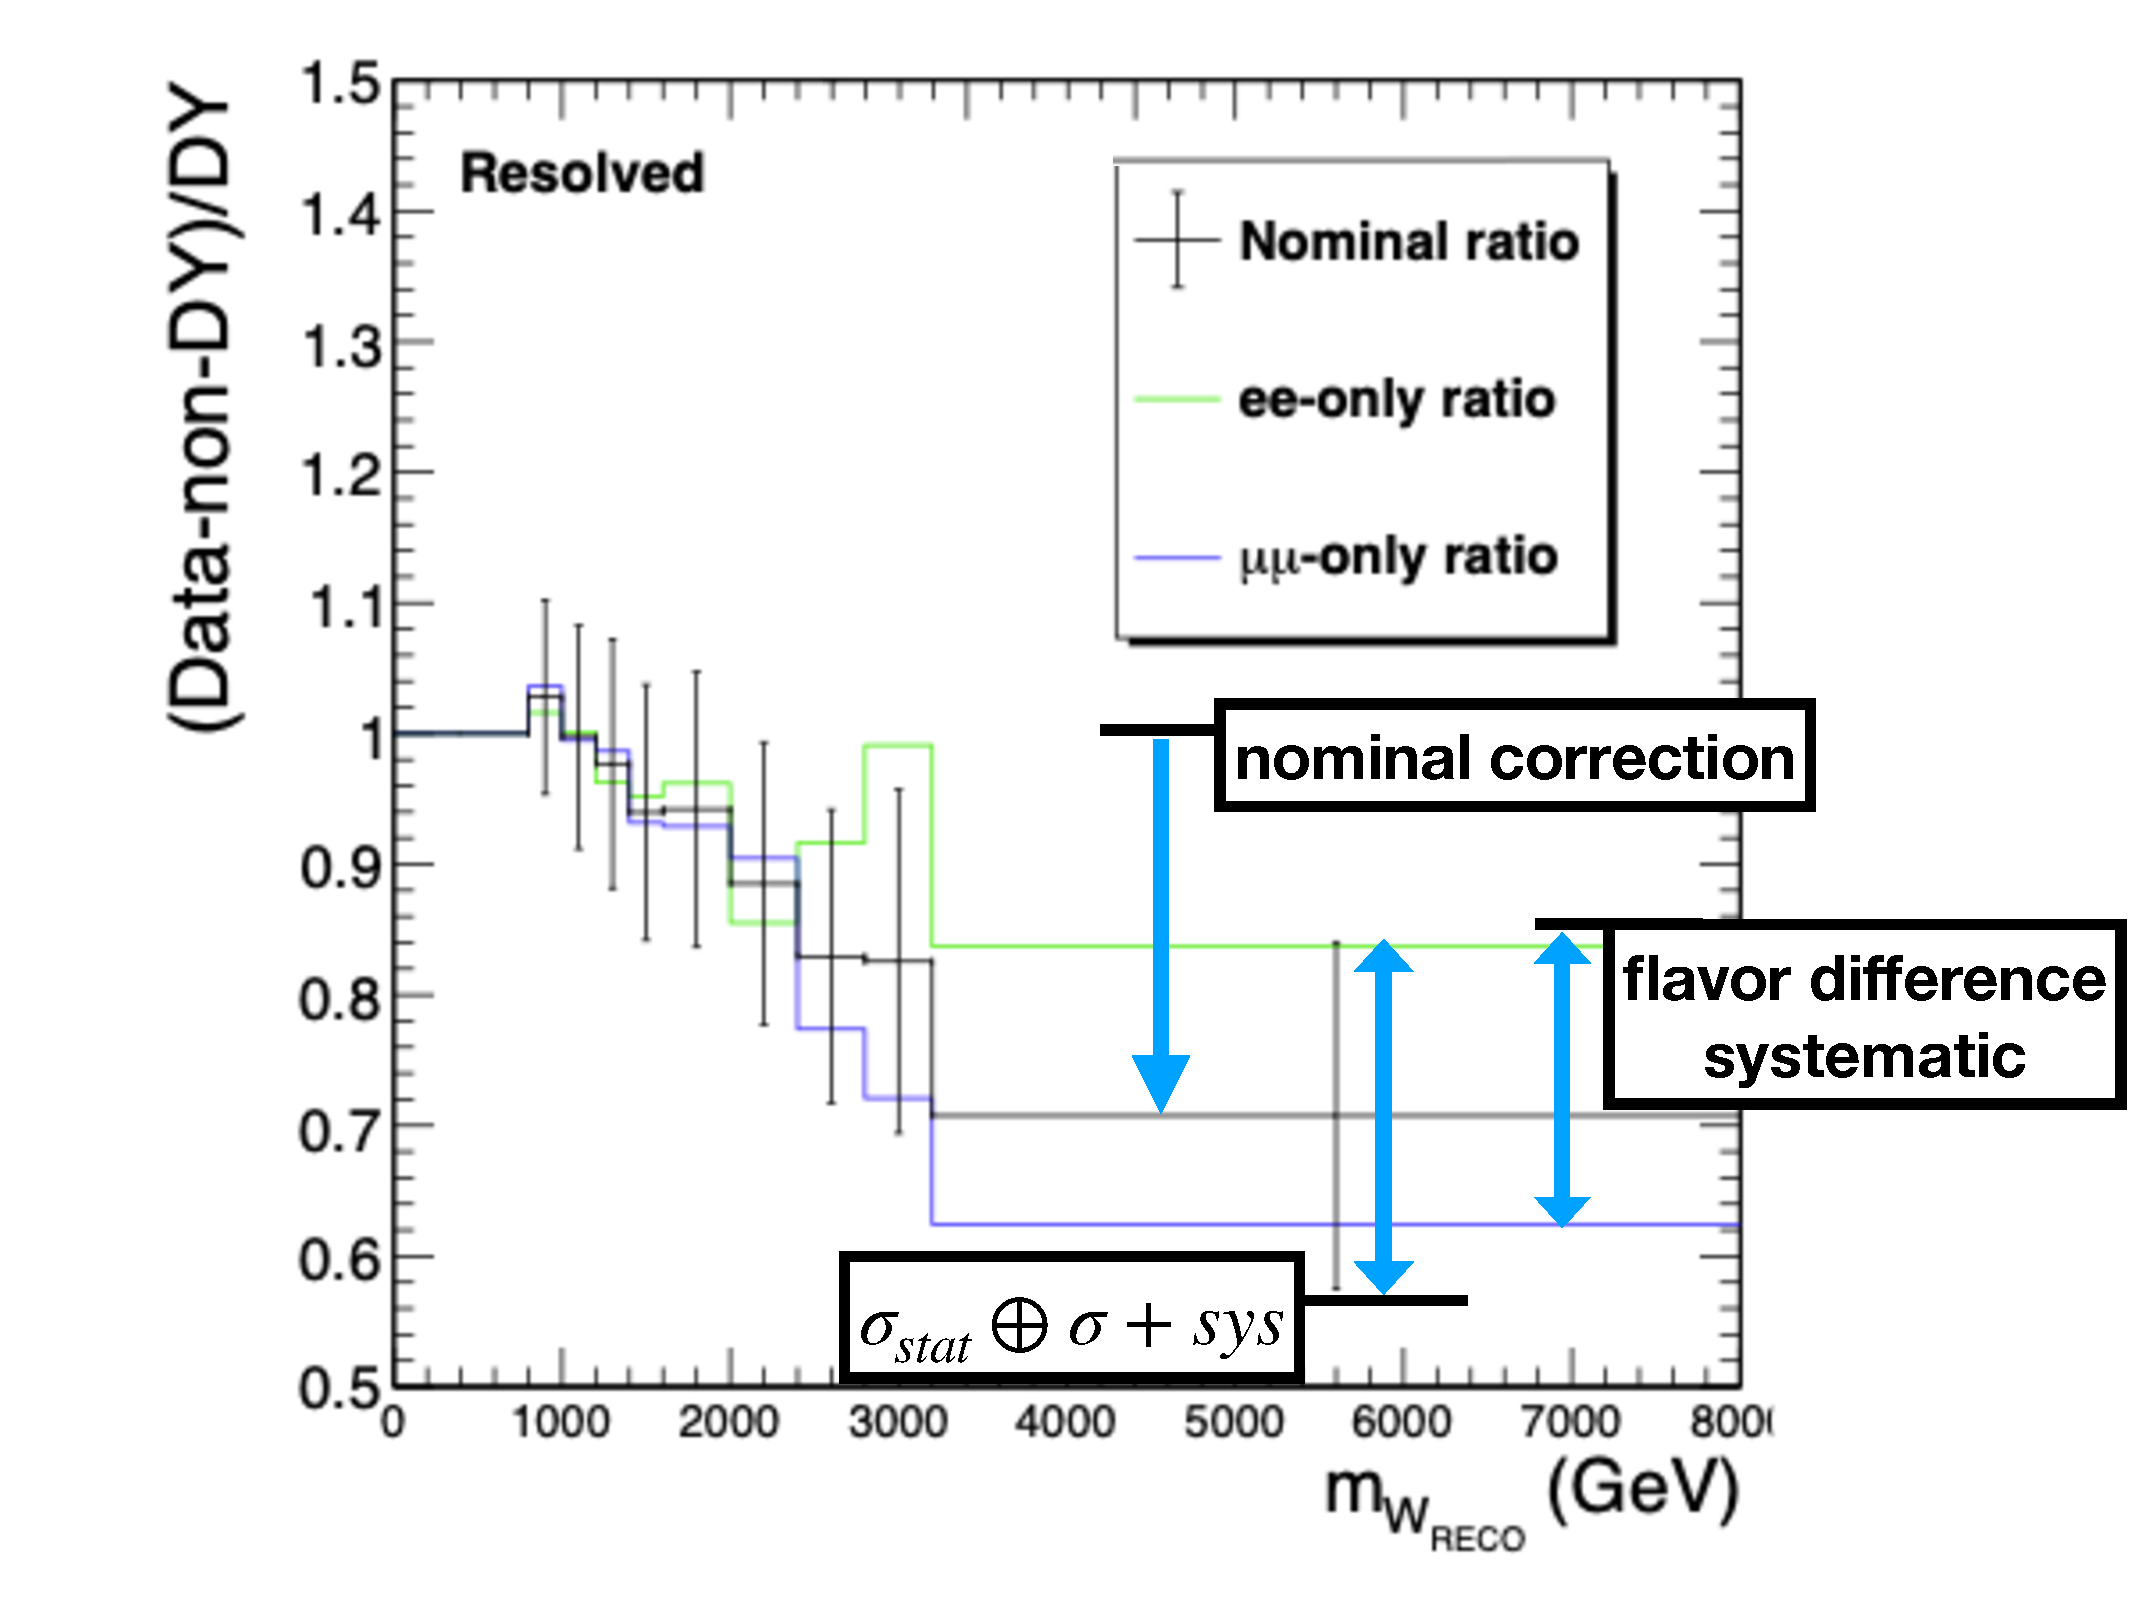
\includegraphics[width=\textwidth]{figures/DYCR_ratio.pdf}

  \caption[Drell-Yan Shape Correction]{
    The ratio of the Drell-Yan calculated in data and in Monte-Carlo in the Z-mass control region for 2018. The nominal value and its uncertainties are labelled.
  }
  \label{fig:DYCR_ratio}
\end{figure}



\subsection{Object Uncertainties}
Systematic differences between simulation and data for the reconstructed jets, electrons, and muons in this analysis are only corrected up to a precision. Beyond this, systematic uncertainties remain for these objects. The event selection is re-run with a parameter (i.e. electron \pt) set at its upper and lower $1\sigma$ bounds. The final $M_{\ell\ell jj}/M_{\ell J}$ mass distribution is then used to see the effect of each parameter's uncertainty.

\begin{itemize}
 \item {\bf LSF scale factor}:
 The most significant object uncertainty comes from the discrepancy between MC and data. Understanding this difference is complicated, as each background and signal produces the reconstructed \NR jet from different processes. This analysis artificially creates a 3-prong, signal-like jet by starting with a hadronically decaying, boosted W (2-prongs) and injecting either an electron or a muon into the event nearby it. This procedure is performed in data and \ttbar MC and the LSF distributions are compared to derive the scale factor for every year individually. The data and simulation distributions of LSF with an injected lepton are shown for both lepton flavors in Fig.~\ref{fig:LSFinjectedLepton}. The difference in efficiency between data and simulation on our LSF selection varies between 0.98 and 1.11 (between all years and lepton flavors) with an uncertainty between 5 and 9 \%. The full results are shown in Table \ref{tab:LSFSF_InjectedSamples}.
 \begin{table}[htbp]
  \caption{
    The LSF scale factors for each year from the injected electron and muon samples.
  }
  \centering
  \label{tab:LSFSF_InjectedSamples}
  \begin{tabular}{ccc}

\hline
Year & Injected $e$ & Injected $\mu$ \\
\hline
2016 & $1.04_{-0.08}^{+0.09}$ & $1.01_{-0.06}^{+0.06}$ \\
2017 & $1.02_{-0.08}^{+0.08}$ & $0.98_{-0.07}^{+0.07}$ \\
2018 & $1.11_{-0.07}^{+0.08}$ & $1.06_{-0.05}^{+0.06}$ \\
\hline
  \end{tabular}
\end{table}

\begin{figure}[!tp]

  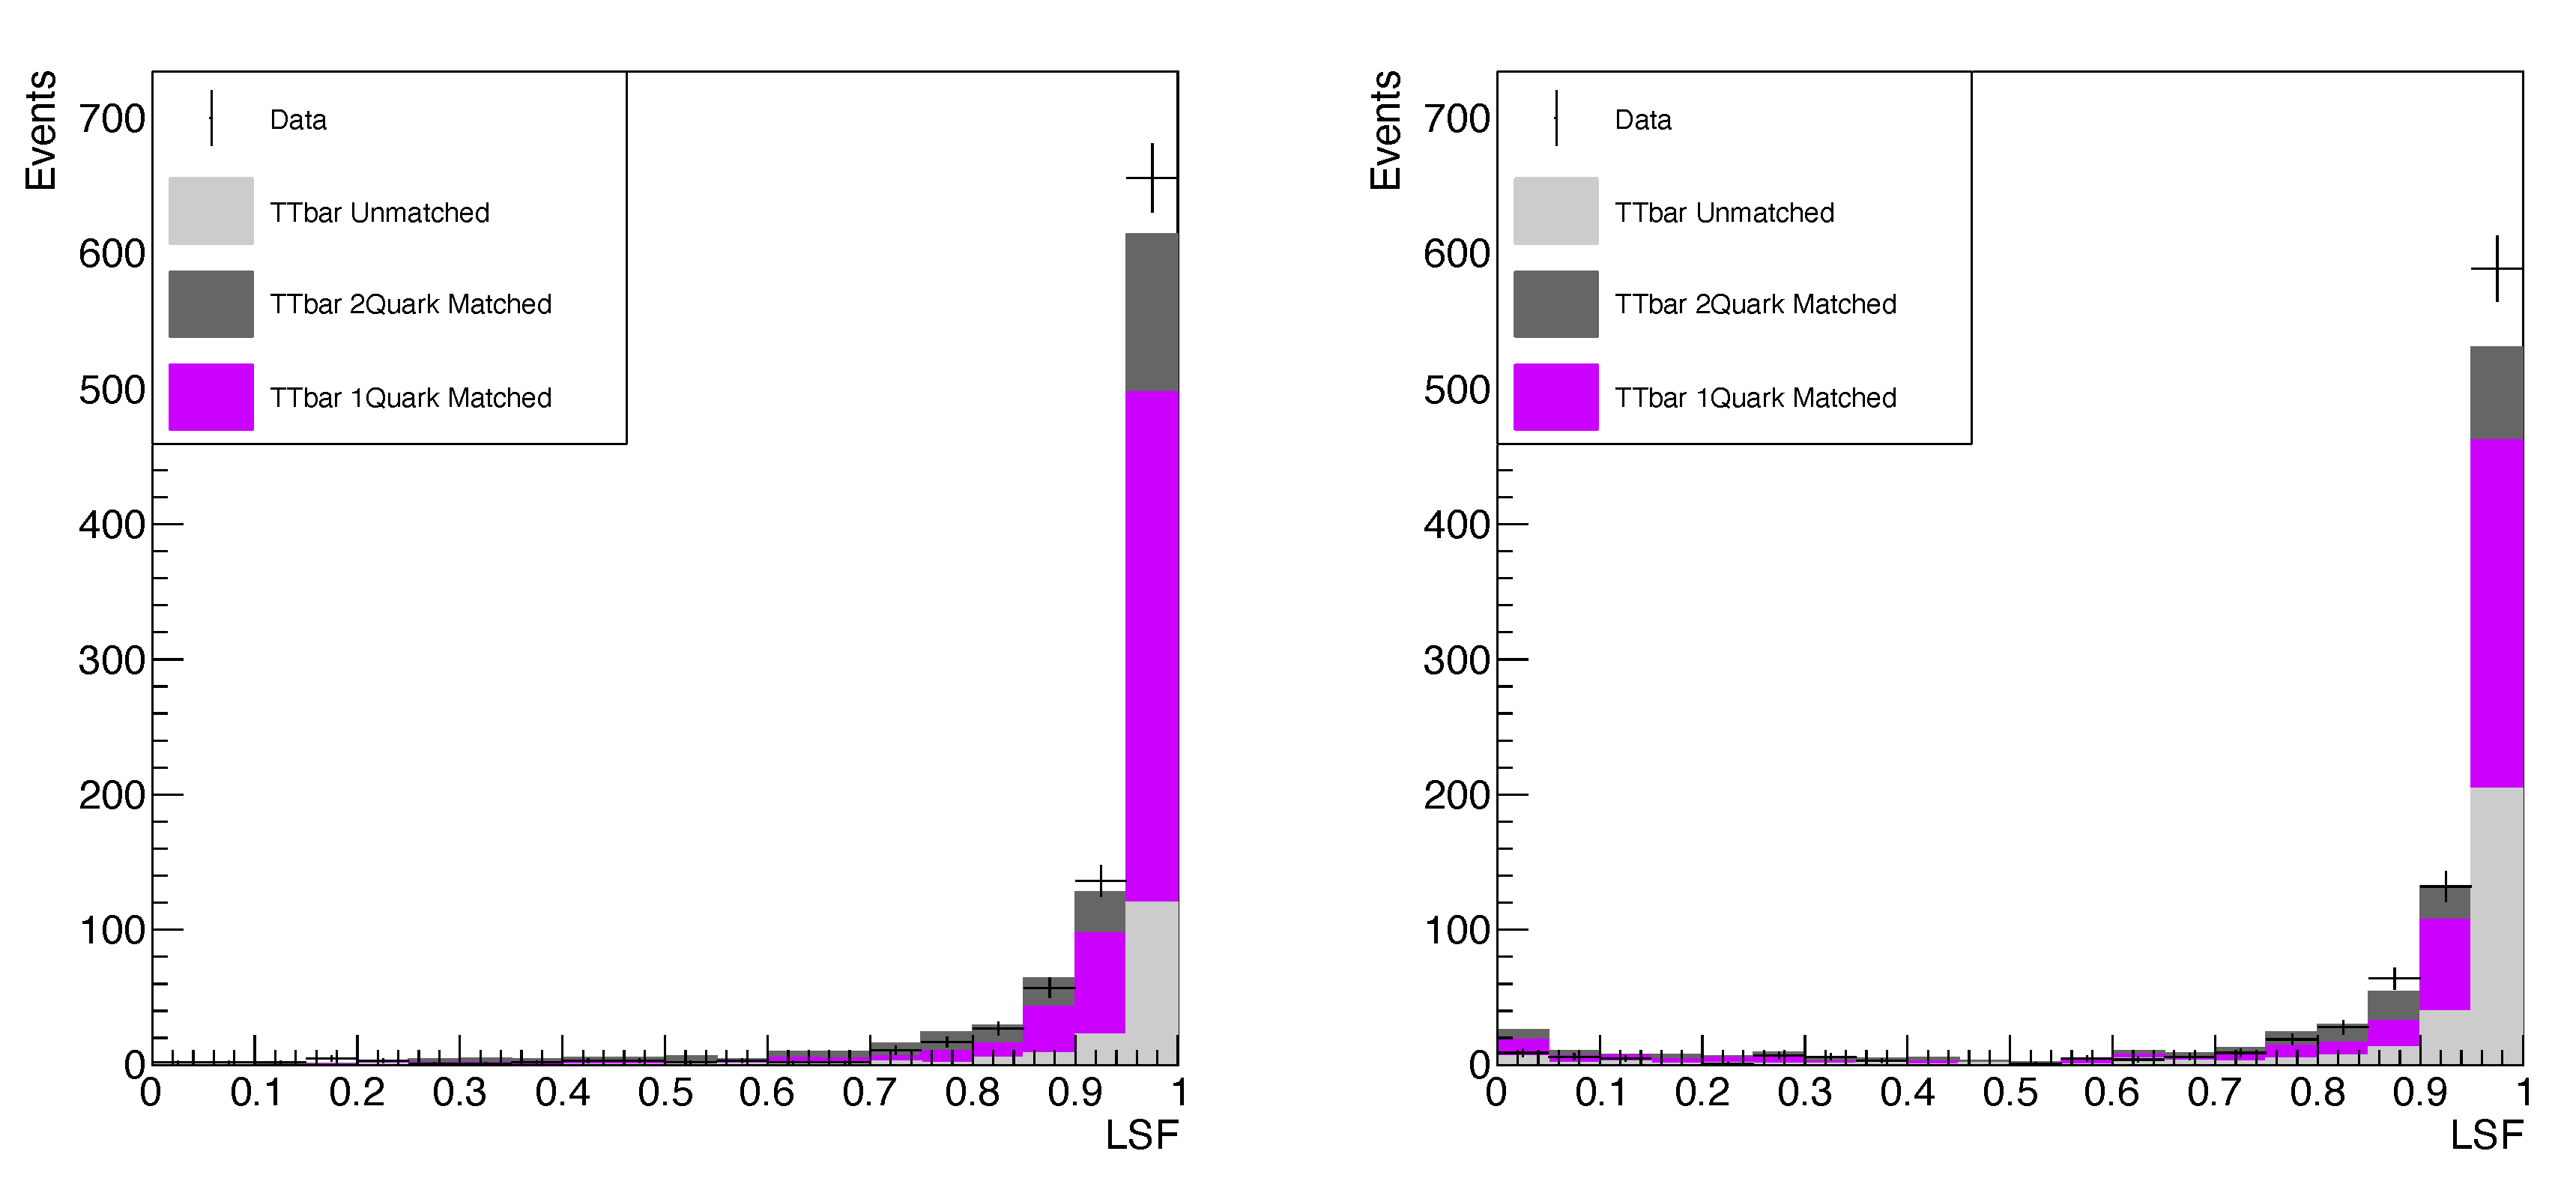
\includegraphics[width=\textwidth]{figures/2018_LSF_Injected_Lepton.pdf}

  \caption[LSF In Data and Simulation]{
    LSF is shown for data and simulation in 2018. The \ttbar simulation is separated in to three categories dependent on how many of the decay-quarks are within the jet cone of 0.8. 
  }
  \label{fig:LSFinjectedLepton}
\end{figure}

\item {\bf Lepton momentum scale and resolution}: The lepton momentum scale uncertainty is computed by varying the momentum of the leptons by their uncertainties.

Neither of the lepton momentum scale and resolution uncertainties are dominant in their respective channels. Each of these corrections apply to the lepton's momentum value, not the event weight itself. As such, a few percent change in their momenta is very unlikely to move the event between analysis bins let alone cause it to fail event requirements.

For muons with $\pt<200\GeV$, the Rochester corrections were applied to the muon momentum,
which removes bias from detector misalignment or magnetic fields~\cite{muonrochcor}.
Systematic uncertainties considered are follows; root-mean-squared (RMS) of pre-generated error sets, difference between results without Z momentum reweighting and variation of profile and fitting mass window,
For muons with $\pt\ge200\GeV$, generalized--endpoint (GE) method~\cite{MuonHighPtRef} was applied,
and the uncertainties on the muon curvature bias are taken from a gaussian distribution.
Muon reconstruction and momentum scale give 0.4--1.0 (0--0.4)~\% and 0.4--2.4 (0.6--3.6)~\% uncertainties in the background estimation in the resolved (boosted) region.

For electrons, we used the MiniAOD V2 energy corrections~\cite{EGMsmearings}, and corresponding uncertainties.
Electron reconstruction~\cite{ELERECOSF}, energy resolution, and energy scale~\cite{EGMsmearings} give 1.0--1.6 (0--0.5)~\%, $<0.1$ ($<0.1$)~\%, and 0.5--1.8 (0.5--2.6)~\% uncertainties in the background estimation in the resolved (boosted) region.
 \item {\bf Lepton trigger and selection}: Discrepancies in the lepton reconstruction, identification, and isolation efficiencies between data and simulation are corrected by applying a scale factor to all the simulated samples. This is explained in Section~\ref{sec:Reconstruction}. For the modified loose electron ID, the discrepancy between data and simulation is calculated as part of our LSF SF.
The scale factors, which depend on the \pt and $\eta$, are varied by $\pm \sigma$ and the change in the yield in the signal region is taken as the systematic. 
Electron identification~\cite{HEEPIDSF,HEEPIDSF2018Prompt} and trigger~\cite{EGammaHLTSFTwiki} give 3.1--3.3 (1.9--2.6)~\% and 0--0.1 (0.2--0.4)~\% uncertainties in the background estimation in the resolved (boosted) region.
Muon identification, isolation and trigger give 0.2--1.2 (0.3--1.4)~\%, 0.1--0.2 (0--0.1)~\%, and 0.1--0.2 (0.6--1.0)~\% uncertainties in the background estimation in the resolved (boosted) region across all regions/years.


  \item {\bf Jet energy scale and resolution}: 
  Like with momentum corrections for leptons, the jet energy scale and resolution apply to the overall jet energy. This does not significantly change the four or two-object mass spectrum.
The versions of JEC and JER are summarized in Table~\ref{tab:JEC} and Table~\ref{tab:JER}
 In order have the resolution in the simulation similar to that in the data the momentum of the jets is smeared as:
   \begin{equation}
     \pt \rightarrow  \mathrm{max} [0, p^{\mathrm{gen}}_{T} + c_{\pm 1 \sigma} \cdot (\pt = p^{\mathrm{gen}}_{T})]
   \end{equation}
in which $c_{\pm 1 \sigma}$ are the data/MC scale factors, which are shifted by $\pm \sigma$. 

This results in a systematic uncertainty of less than $1\%$ for all masses.

 
\end{itemize}

\subsection{Event Uncertainties}
There are several uncertainties related to event weights applied to background and signal simulations. Their effects are generally small, and vary in application depending on the uncertainty.
\begin{itemize}

  \item {\bf Integrated luminosity}: The systematic uncertainty on the integrated luminosity are $2.5\%$, $2.3\%$, and $2.5\%$ for 2016, 2017 and 2018, respectively~\cite{CMS-PAS-LUM-17-001,CMS-PAS-LUM-17-004,CMS-PAS-LUM-18-002}. The integrated luminosity is used to scale background and signal simulations for them to be compared to data. Each of the major backgrounds has additional scaling to data in the simultaneous fit making this uncertainty effectively irrelevant for backgrounds. Signal simulations, however, are scaled by luminosity and otherwise uncorrected to create the two-dimensional \WRNR mass limits. It remains, however, not a dominant uncertainty in those limits.

  \item {\bf Pileup}: The number of collision vertices in every event varies. This distribution is modeled in simulation and compared with data for each year. An uncertainty is estimated by varying the minimum bias cross section of pp collisions at 13 TeV. This uncertainty is not very significant.

  \item {\bf Theoretical uncertainties}: For signal simulation, only the uncertainties on the rate and acceptance of the signal are derived from the variation of the QCD scale, the parton distribution functions (PDFs) and \alpS.
  The PDF and \alpS uncertainties for the \MADGRAPH signal samples are estimated from the standard deviation of the weights from the PDF errorsets provided in the NNPDF3.1 parton distribution set.
  The procedure for estimating the uncertainties associated with the PDF follows the recommendations issued by the PDF4LHC group~\cite{PDF4LHC}.
  
  \item {\bf Pre-firing probabilities}:
Followed by the recommendation pre-firing study group in CMS, a 20~\% systematic uncertainty is applied in addition to the statistical uncertainty on the pre-firing scale factor.

\end{itemize}

\subsection{Multi-Year Correlations}
For this analysis, the three main data taking years of Run II are analyzed. Each year changes in the detector and \LHC conditions occurred, some subtle, and others less so (like the HEM failure in 2018). Collision events between years are generally considered uncorrelated. However, as a conservative default, systematic uncertainties considered in this analysis correlate between years, and the statistical uncertainty of events in different years are completely uncorrelated. A few systematic uncertainties are uncorrelated. A full list of all the uncertainties and the range of their effects on event yields in different signal regions and years is shown in Table~\ref{tab:systUnc}


\section{Model Inputs}
Having covered the background estimations and the diverse uncertainties in the analysis, all of the distributions used as inputs to the fitting and hypothesis testing process are shown here. The flavor sideband, Drell-Yan, and lepton-flavor signal regions are shown with each of the years shown independently.

\begin{figure}[htbp]
  \centering

  \includegraphics[width=0.45\textwidth]{figures/2016/AfterZPtReweight_AfterDYNorm_AfterDYReshape_WRCand_Mass_HNWR_SingleElectron_Resolved_DYCR.pdf}
  \hspace{0.01\textwidth}
  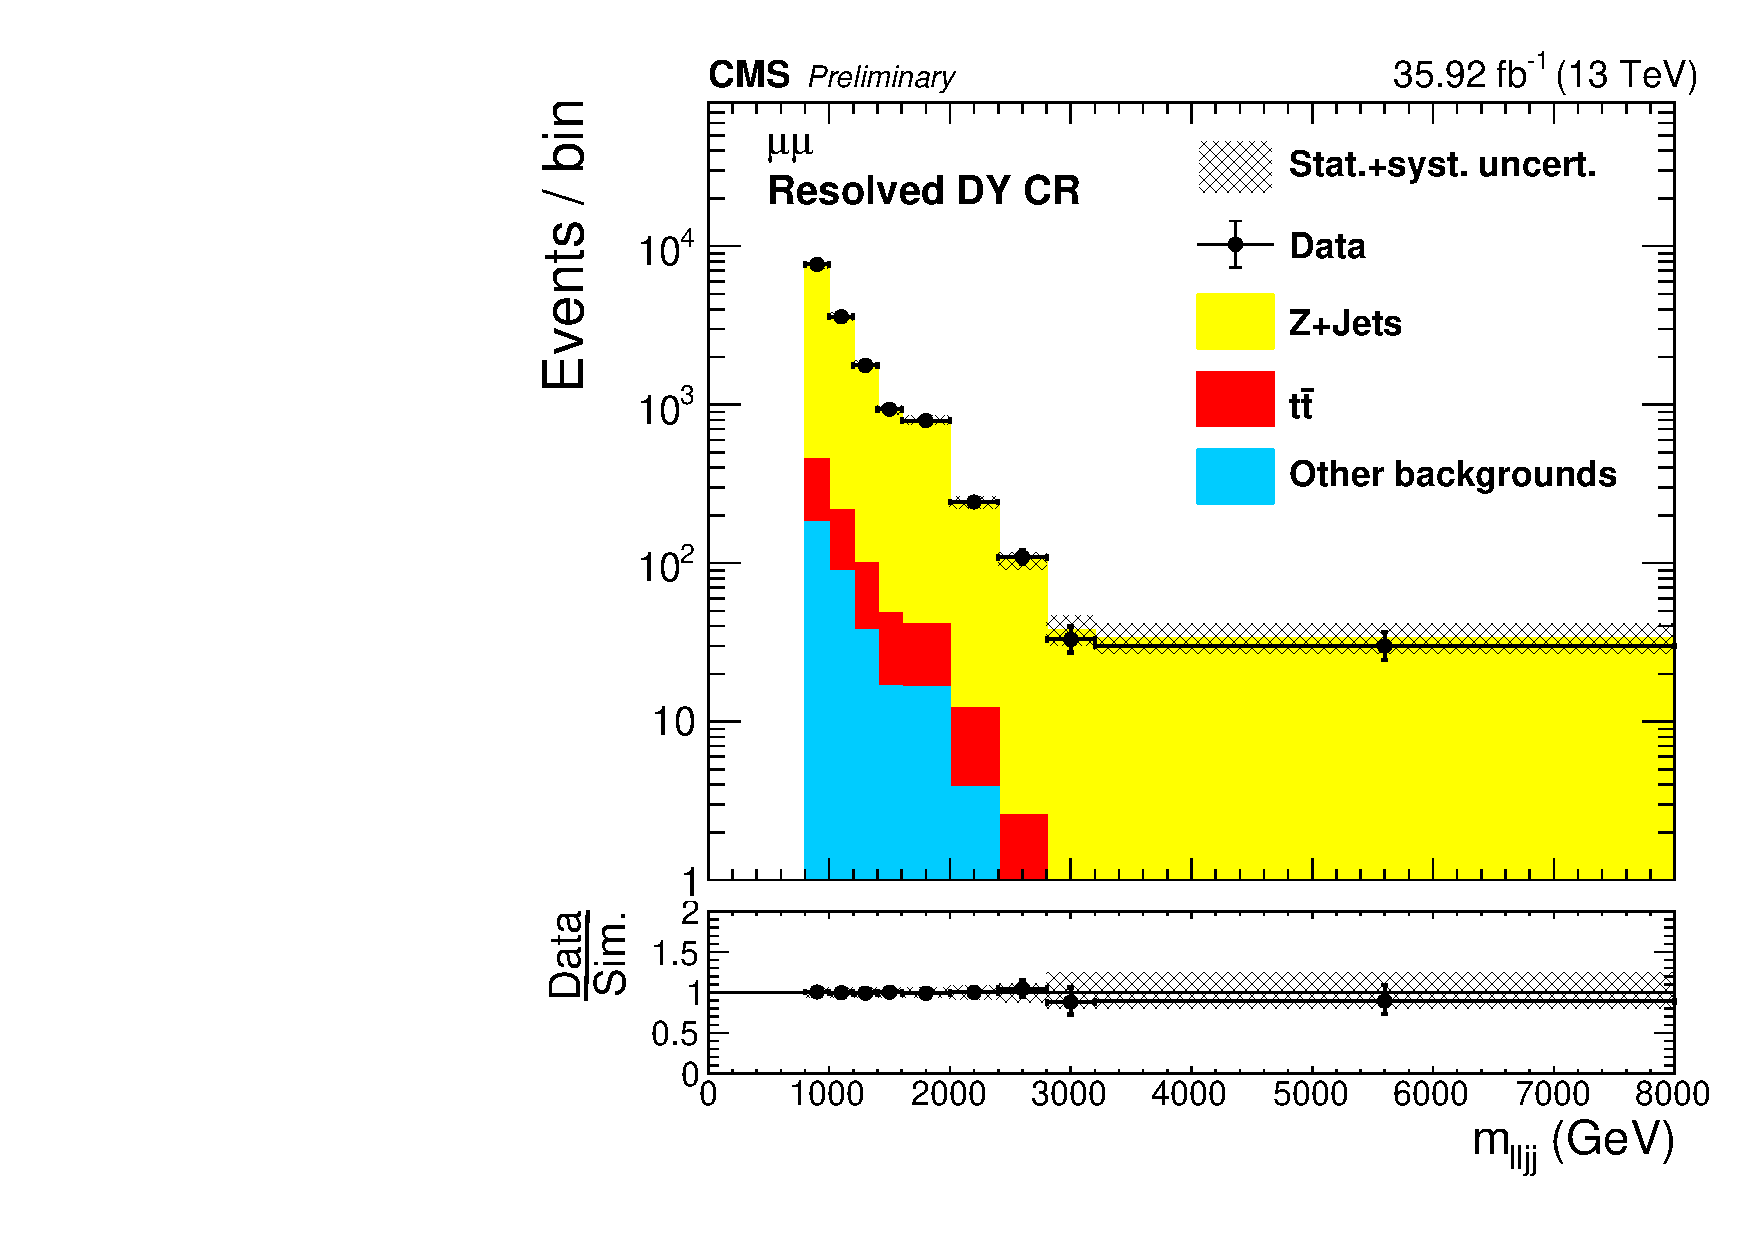
\includegraphics[width=0.45\textwidth]{figures/2016/AfterZPtReweight_AfterDYNorm_AfterDYReshape_WRCand_Mass_HNWR_SingleMuon_Resolved_DYCR.pdf}
  \vspace{0.01\textwidth}

  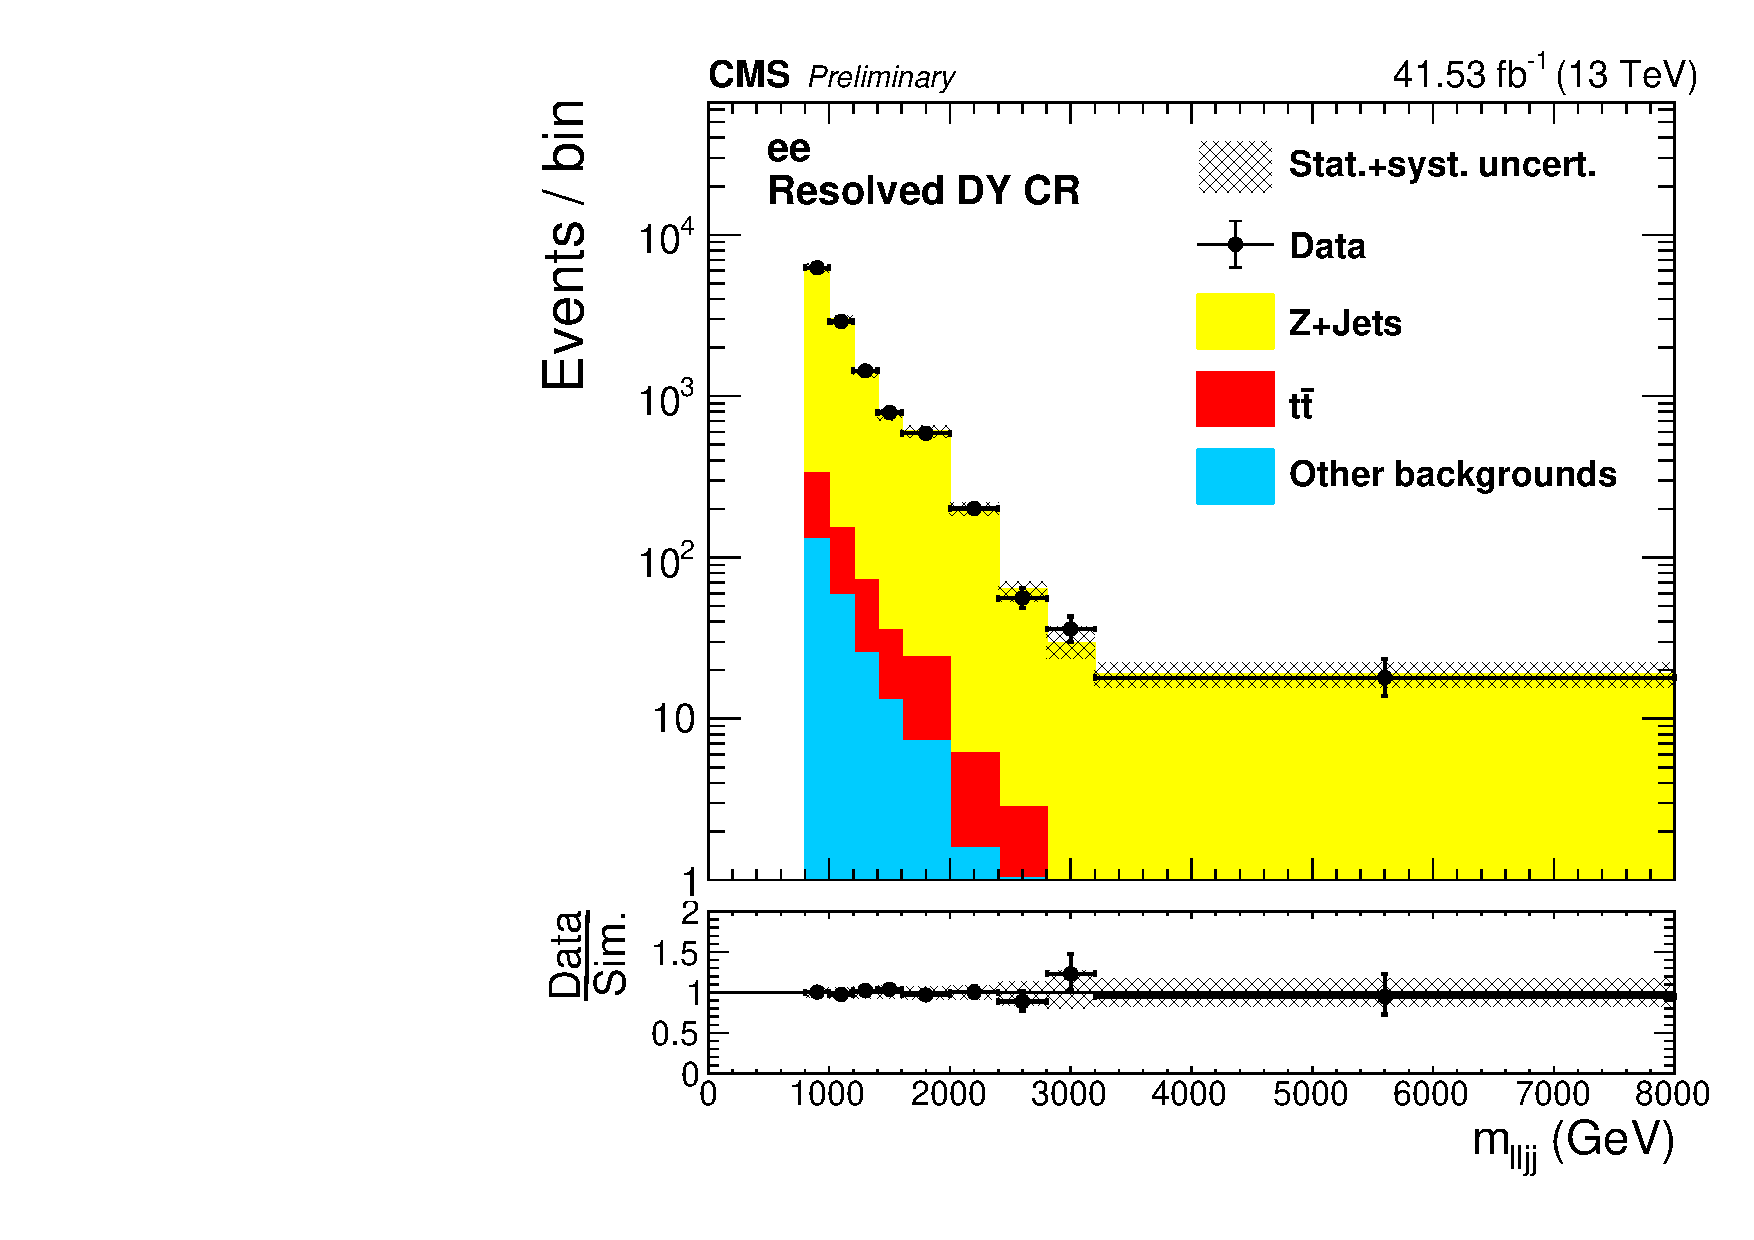
\includegraphics[width=0.45\textwidth]{figures/2017/AfterZPtReweight_AfterDYNorm_AfterDYReshape_WRCand_Mass_HNWR_SingleElectron_Resolved_DYCR.pdf}
  \hspace{0.01\textwidth}
  \includegraphics[width=0.45\textwidth]{figures/2017/AfterZPtReweight_AfterDYNorm_AfterDYReshape_WRCand_Mass_HNWR_SingleMuon_Resolved_DYCR.pdf}
  \vspace{0.01\textwidth}

  \includegraphics[width=0.45\textwidth]{figures/2018/AfterZPtReweight_AfterDYNorm_AfterDYReshape_WRCand_Mass_HNWR_SingleElectron_Resolved_DYCR.pdf}
  \hspace{0.01\textwidth}
  \includegraphics[width=0.45\textwidth]{figures/2018/AfterZPtReweight_AfterDYNorm_AfterDYReshape_WRCand_Mass_HNWR_SingleMuon_Resolved_DYCR.pdf}


  \topcaption{
    The $m(\ell \ell \jet \jet)$ in the low $m_{\ell\ell}$ Resolved control regions, after applying the DY ratio.
    Results for dielectron (dimuon) channel is shown on the left (right), for 2016 (upper), 2017 (middle) and 2018 (lower).
  }
  \label{fig:AfterZPtReweight_AfterDYNorm_AfterDYReshape_WRCand_Mass_Resolved_DYCR}
\end{figure}

\begin{figure}[htbp]
  \centering

  \includegraphics[width=0.45\textwidth]{figures/2016/AfterZPtReweight_AfterDYNorm_AfterDYReshape_WRCand_Mass_HNWR_SingleElectron_Boosted_DYCR.pdf}
  \hspace{0.01\textwidth}
  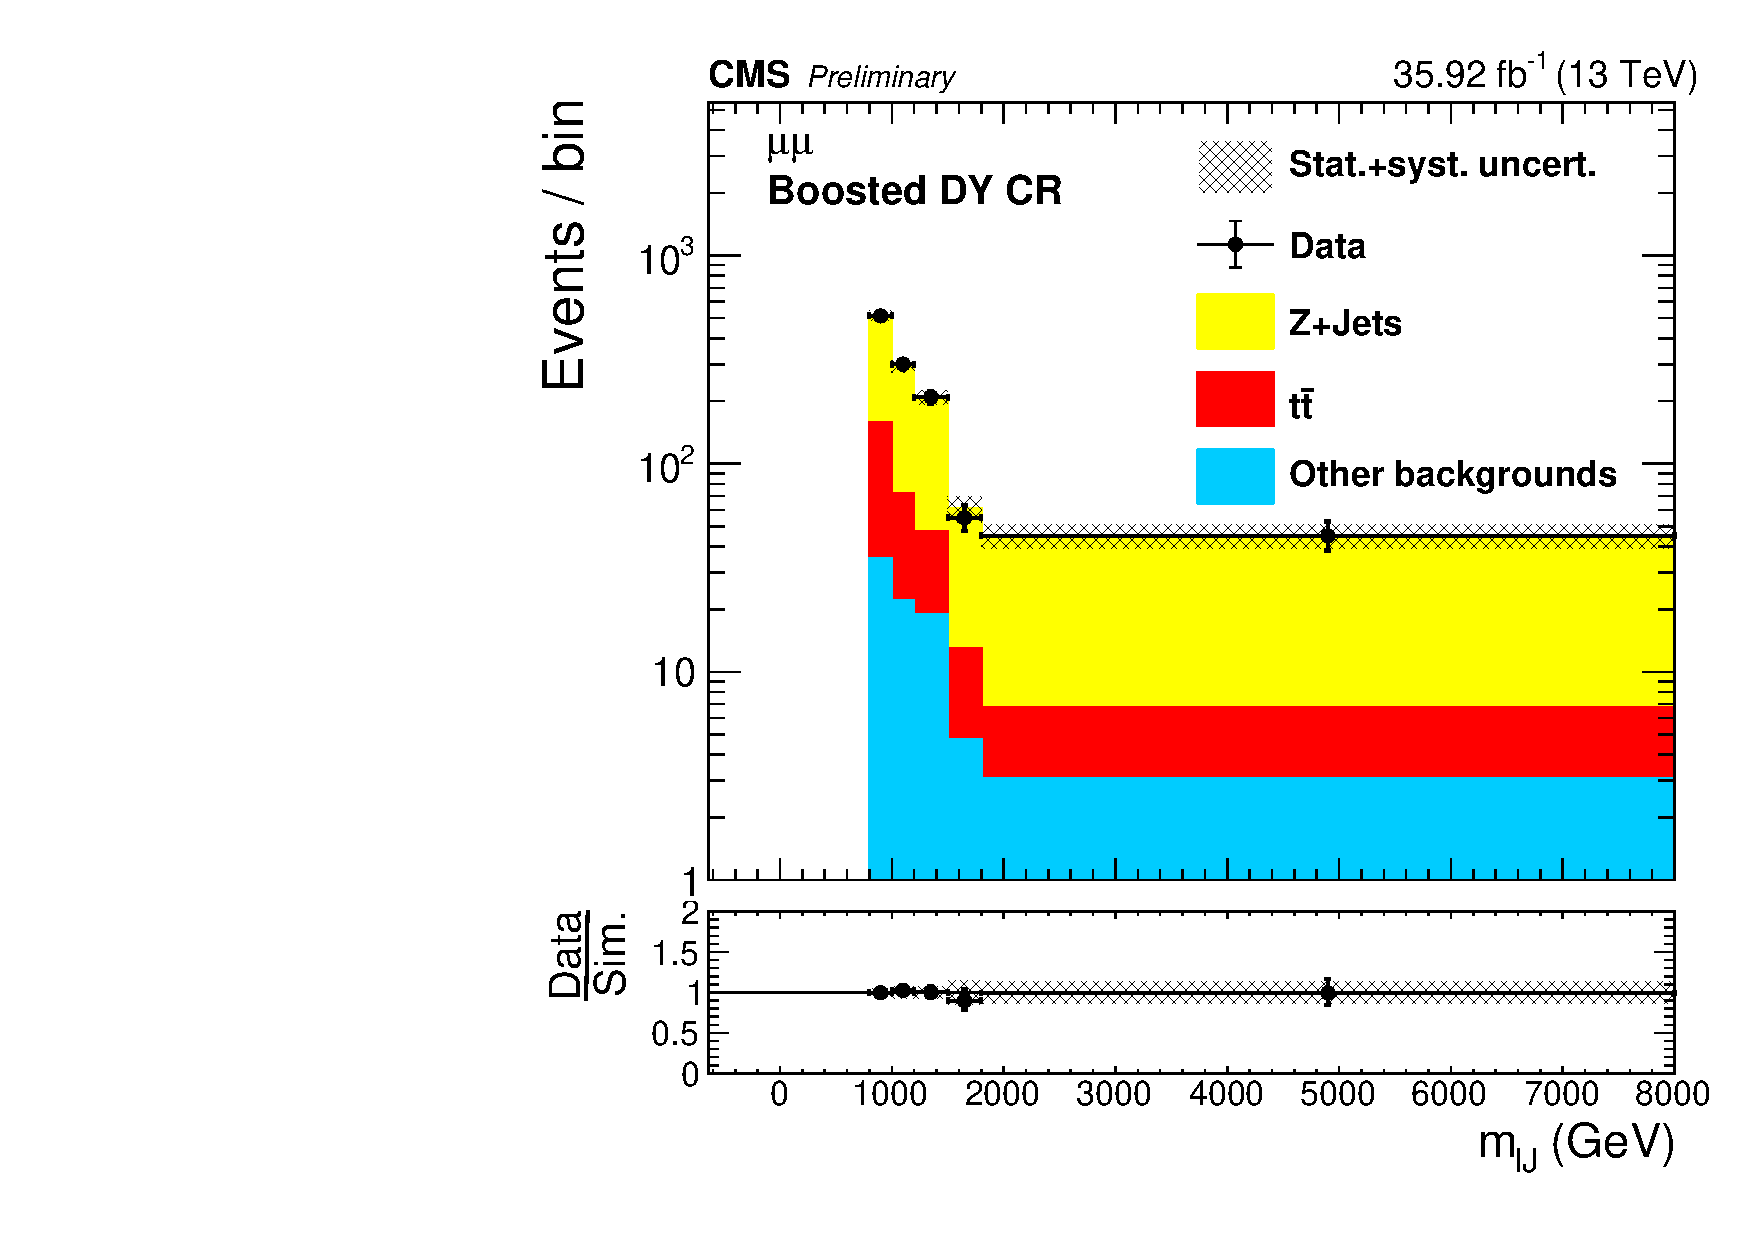
\includegraphics[width=0.45\textwidth]{figures/2016/AfterZPtReweight_AfterDYNorm_AfterDYReshape_WRCand_Mass_HNWR_SingleMuon_Boosted_DYCR.pdf}
  \vspace{0.01\textwidth}

  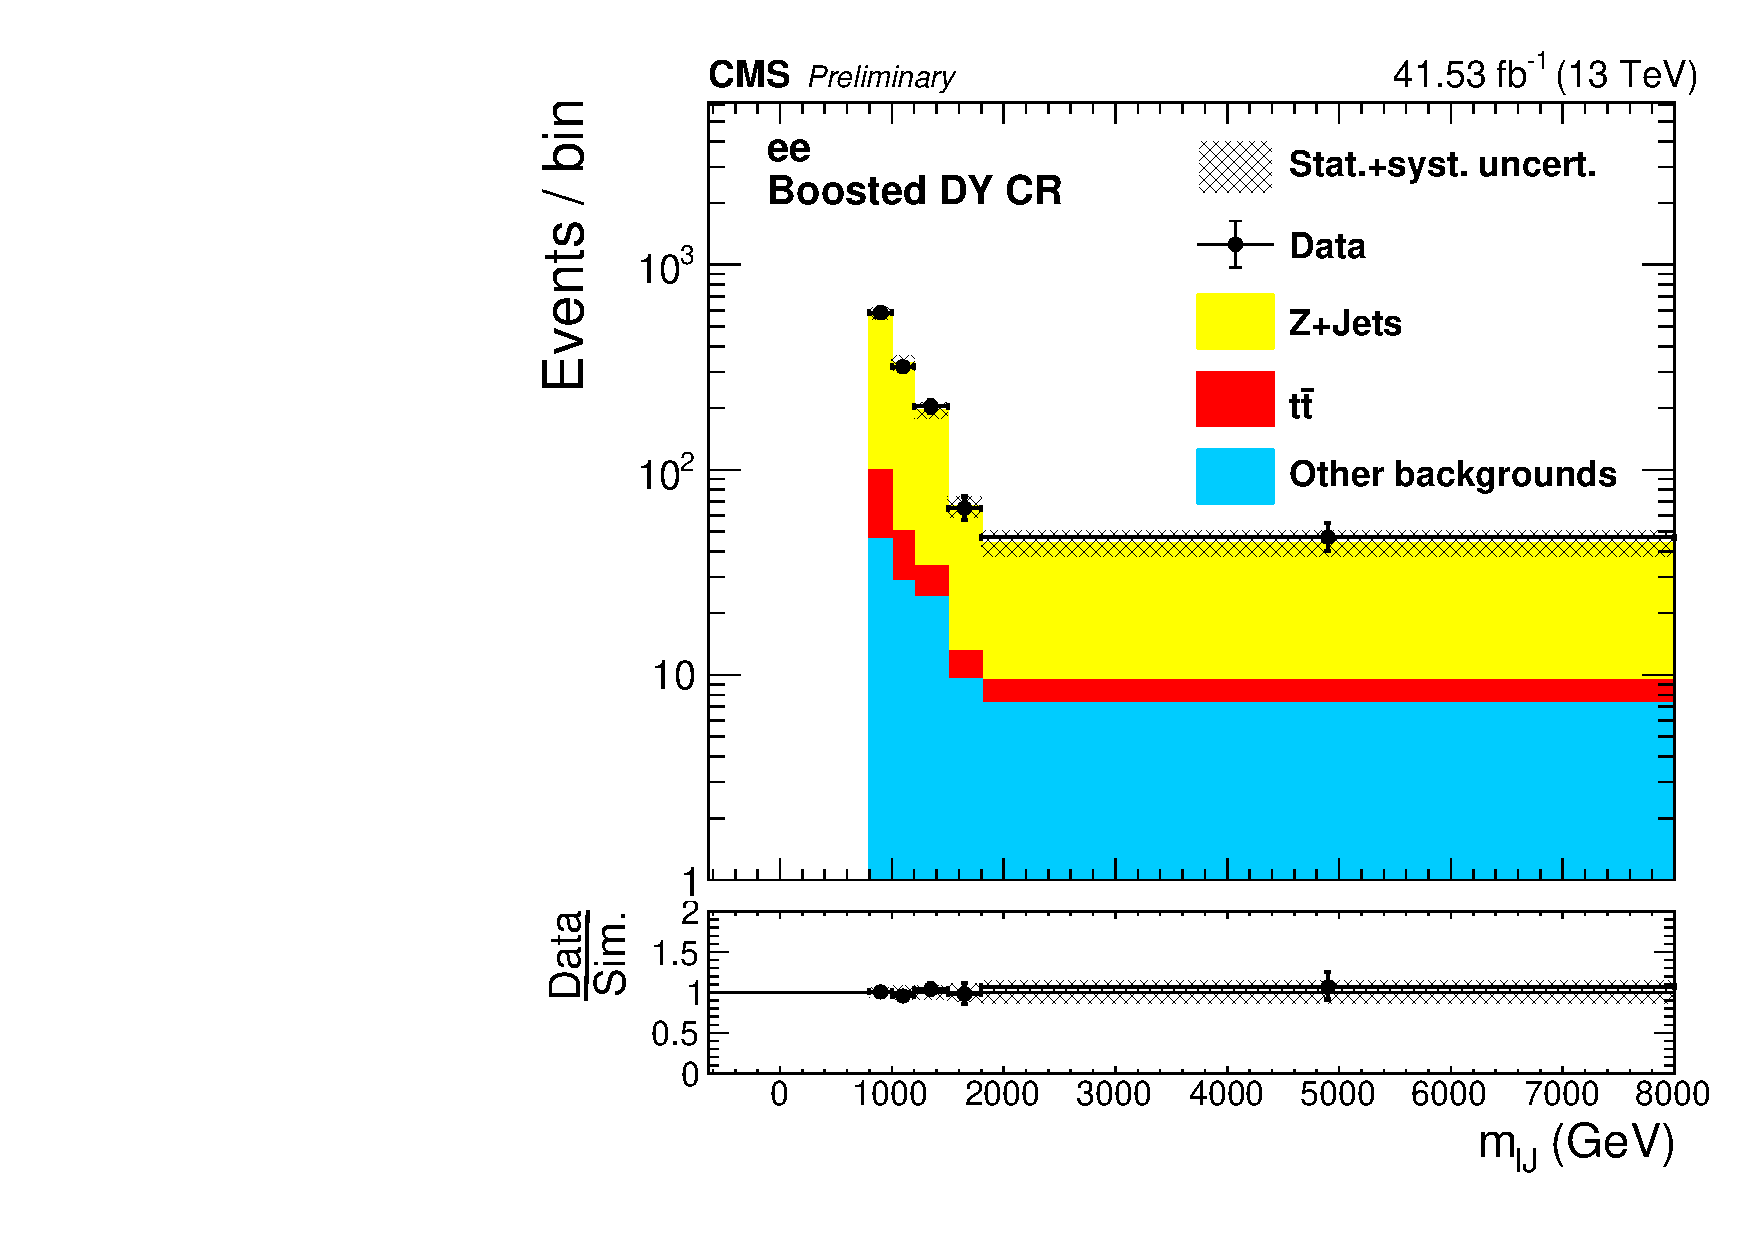
\includegraphics[width=0.45\textwidth]{figures/2017/AfterZPtReweight_AfterDYNorm_AfterDYReshape_WRCand_Mass_HNWR_SingleElectron_Boosted_DYCR.pdf}
  \hspace{0.01\textwidth}
  \includegraphics[width=0.45\textwidth]{figures/2017/AfterZPtReweight_AfterDYNorm_AfterDYReshape_WRCand_Mass_HNWR_SingleMuon_Boosted_DYCR.pdf}
  \vspace{0.01\textwidth}

  \includegraphics[width=0.45\textwidth]{figures/2018/AfterZPtReweight_AfterDYNorm_AfterDYReshape_WRCand_Mass_HNWR_SingleElectron_Boosted_DYCR.pdf}
  \hspace{0.01\textwidth}
  \includegraphics[width=0.45\textwidth]{figures/2018/AfterZPtReweight_AfterDYNorm_AfterDYReshape_WRCand_Mass_HNWR_SingleMuon_Boosted_DYCR.pdf}


  \topcaption{
    The $m(\ell \Jet)$ of dilepton in the low $m_{\ell\ell}$ boosted control regions, after applying the DY ratio.
    Results for dielectron (dimuon) channel is shown on the left (right), for 2016 (upper), 2017 (middle) and 2018 (lower).
  }
  \label{fig:AfterZPtReweight_AfterDYNorm_AfterDYReshape_WRCand_Mass_Boosted_DYCR}
\end{figure}




\begin{table}[htbp]%
  \centering
 
  

\resizebox{\textwidth}{!}{%
  \begin{tabular}{lcccccc}
\hline
\multirow{2}{*}{Source} & \multirow{2}{*}{Bkgd./Signal process} &\multirow{2}{*}{Year-to-year treatment} & $ee$ bkgd. & $ee$ signal & $\mu\mu$ bkgd. & $\mu\mu$ signal \\
                        &                                       &     &  (\%)           & (\%)            & (\%)           & (\%) \\
\hline

Integrated luminosity & All bkgd./Signal & Uncorrelated & 2.3--2.5 (2.3--2.5) & 2.3--2.5 (2.3--2.5) & 2.3--2.5 (2.3--2.5) & 2.3--2.5 (2.3--2.5) \\
Jet energy resolution & All bkgd./Signal & Uncorrelated & 0.5--1.4 (0.7--2.0) & 0--0.9 (0--0.6) & 0.2--1.2 (0.2--1.2) & 0--0.7 (0--1.0) \\
Jet energy scale & All bkgd./Signal & Correlated & 1.9--4.2 (0.9--2.0) & 0--0.4 (0--0.3) & 2.1--3.4 (0.6--1.0) & 0--0.1 (0--0.4) \\
Muon reconstruction & All bkgd./Signal & Correlated & --- & --- & 0.4--1.0 (0.3--0.8) & 5.8--36.8 (5.9--30.4) \\
Muon momentum scale & All bkgd./Signal & Correlated & --- & --- & 0.4--2.5 (0.5--3.6) & 0.1--0.2 (0.1--0.6) \\
Muon identification & All bkgd./Signal & Correlated & --- & --- & 0.2--1.2 (0.1--0.6) & 0.2--1.1 (0.1--0.5) \\
Muon isolation & All bkgd./Signal & Correlated & --- & --- & 0.1--0.2 (0--0.1) & 0.1--0.2 (0--0.1) \\
Muon trigger & All bkgd./Signal & Uncorrelated & --- & --- & 0.1--0.2 (0.1--0.3) & 0.6--1.5 (0.5--1.3) \\
Electron reconstruction & All bkgd./Signal & Correlated & 1.0--1.6 (0.5--0.8) & 0.8--1.4 (0.4--0.8) & --- & --- \\
Electron energy resolution & All bkgd./Signal & Correlated & $<0.1$ ($<0.1$) & $<0.1$ ($<0.1$) & --- & --- \\
Electron energy scale & All bkgd./Signal & Correlated & 0.5--1.8 (0.5--2.3) & 0--0.3 (0--0.4) & --- & --- \\
Electron identification & All bkgd./Signal & Correlated & 3.0--3.2 (1.8--1.9) & 4.1--4.4 (2.1--2.5) & --- & --- \\
Electron trigger & All bkgd./Signal & Uncorrelated & 0--0.1 (0.2--0.4) & $<0.1$ (0.1--0.2) & --- & --- \\
LSF scale factor & All bkgd./Signal & Uncorrelated & ---~(7.2--8.7) & ---~(7.2--8.7) & ---~(5.7--7.1) & ---~(5.7--7.1) \\
Pileup modeling & All bkgd./Signal & Correlated & 0.2--1.1 (0.5--1.1) & 0.1--1.1 (0--2.2) & 0.3--0.5 (0.2--1.1) & 0.1--1.9 (0.1--2.4) \\
Prefire reweighting & All bkgd./Signal & Correlated & 0--1.4 (0--1.1) & 0--0.9 (0--1.0) & 0--0.5 (0--0.4) & 0--0.5 (0--0.2) \\
Z \pt & \ZgJ & Correlated & 2.6--3.3 (2.7--3.5)& --- & 2.7--3.1 (2.8--3.4)& --- \\
DY reshape & \ZgJ & Uncorrelated & 3.9--4.6 (4.6--5.5)& --- & 4.0--4.6 (4.6--5.5)& --- \\
PDF error & Signal & Correlated & --- & 3.7--10.4 (11.0--38.7) & --- & 4.7--10.7 (12.5--43.3) \\
\alpS & Signal & Correlated & --- & 0--0.1 (0.1--0.9) & --- & 0--0.1 (0--1.1) \\
renorm./factorization scales & Signal & Correlated & --- & 0--0.1 (0.3--2.3) & --- & 0--0.1 (2.1--2.9) \\
\hline
  \end{tabular}
  }
  \caption{
Summary of the relative systematic uncertainties in signal and \ZgJ background.
The uncertainties are given for the resolved (boosted) SR.
The numbers for signal is obtained for $m_{\WR}=\SI{5}{TeV}$.
The range given for each systematic uncertainty source covers the variation across the years.
  }

  \label{tab:systUnc}

\end{table}%


%We assigned a systematic uncertainty of 20~\% (30~\%) is assigned for the resolved (boosted) signal region which covers the largest discrepancy in the low invariant mass control region (App.~\ref{appendix_EMuSyst}).